\listfiles
\documentclass{elsarticle}
%\documentclass[final,5p,times,twocolumn]{elsarticle}
\usepackage{hyperref}
\pdfstringdefDisableCommands{%
  \def\corref#1{}%
}
\usepackage{tabularx}
\usepackage{adjustbox}
\usepackage{afterpage}
\usepackage{algorithm,algorithmic}
\usepackage{amsfonts}
\usepackage{amsmath,amssymb}
\usepackage{booktabs}
\usepackage{color,colortbl}
\usepackage{comment}
\usepackage{float}
\usepackage{graphicx}
\usepackage{subcaption}
\usepackage{mathrsfs}
\usepackage{multirow}
\usepackage{pdflscape}
\usepackage{lineno,hyperref}
\usepackage{longtable}
\usepackage{siunitx}
\usepackage{tikz}
\usepackage{svg}
\usepackage{ulem}
\usepackage{booktabs}
\usepackage{multirow}

\modulolinenumbers[5]

\newcommand{\No}[1]{{\color{red}\sout{#1}}}
\newcommand{\Si}[1]{{\color{blue}#1}}

\usepackage{pgfplots}
\pgfplotsset{compat=1.9}
\usepgfplotslibrary{external}
\tikzexternalize

\newcommand{\diff}{\textit{diff}}
\newcommand{\gris}[1]{\textcolor{lightgray}{#1}}

\journal{Journal's name}

%%%%%%%%%%%%%%%%%%%%%%%
%% Elsevier bibliography styles
%%%%%%%%%%%%%%%%%%%%%%%
%% To change the style, put a % in front of the second line of the current style and
%% remove the % from the second line of the style you would like to use.
%%%%%%%%%%%%%%%%%%%%%%%

%% Numbered
%\bibliographystyle{model1-num-names}

%% Numbered without titles
%\bibliographystyle{model1a-num-names}

%% Harvard
%\bibliographystyle{model2-names.bst}\biboptions{authoryear}

%% Vancouver numbered
%\usepackage{numcompress}\bibliographystyle{model3-num-names}

%% Vancouver name/year
%\usepackage{numcompress}\bibliographystyle{model4-names}\biboptions{authoryear}

%% APA style
%\bibliographystyle{model5-names}\biboptions{authoryear}

%% AMA style
%\usepackage{numcompress}\bibliographystyle{model6-num-names}

%% `Elsevier LaTeX' style
%\bibliographystyle{elsarticle-num}
%%%%%%%%%%%%%%%%%%%%%%%

\begin{document}

\begin{frontmatter}

\title{Exploration of Bioinspired Algorithms in Multithreshold Image Segmentation for Medical Images}

%\tnotetext[mytitlenote]{Fully documented templates are available in the elsarticle package on % %\href{http://www.ctan.org/tex-archive/macros/latex/contrib/elsarticle}{CTAN}.
%}

%% or include affiliations in footnotes:
%\author[mymainaddress,mysecondaryaddress]{Elsevier Inc}
%\ead[url]{www.elsevier.com}

%\author[mysecondaryaddress]{Global Customer Service\corref{mycorrespondingauthor}}
%\cortext[mycorrespondingauthor]{Corresponding author}
%\ead{support@elsevier.com}

%\address[mymainaddress]{1600 John F Kennedy Boulevard, Philadelphia}
%\address[mysecondaryaddress]{360 Park Avenue South, New York}

\author{Fernando Ramírez\corref{cor}}
\cortext[cor]{Corresponding author}
\ead{fernando.ramirezs@postgrado.uv.cl}

\author{Emilio Flores}
\ead{emilio.flores@postgrado.uv.cl}

\author{Rodrigo Olivares}
\ead{rolivares@uv.cl}

\address{Escuela de Ingenier\'ia Inform\'atica, Universidad de Valpara\'iso, Valpara\'iso, Chile.}

\begin{abstract}
\noindent El cerebro es esencial para el funcionamiento humano, es vulnerable a múltiples patologías, incluidos accidentes cerebrovasculares, tumores cerebrales y otros trastornos que comprometen su estructura y función. Las imágenes médicas obtenidas a través de técnicas que utilizan radiaciones ionizantes o resonancia magnética (MRI) son fundamentales para evaluar estas condiciones.

\noindent En este contexto, la segmentación de imágenes del cerebro se convierte en una herramienta crítica para delinear con precisión las estructuras anatómicas y patológicas, facilitando tanto el diagnóstico como la planificación terapéutica. La segmentación se lleva a cabo de forma no supervisada utilizando técnicas como la entropía de Kapur, entropía de Tsallis y el método Otsu multinivel, apoyadas en algoritmos de optimización metaheurística que buscan determinar los umbrales de segmentación más efectivos.

\noindent Este estudio realiza una comparativa exhaustiva de ocho algoritmos de optimización metaheurística: RSA, OPA, BES, GWO, HBA, CSA, HHO y TSO. Evalúa su eficacia utilizando métricas clave como la función de aptitud, el Peak Signal-to-Noise Ratio (PSNR) y el Structural Similarity Index (SSIM). Una de las principales innovaciones de esta investigación es la aplicación de estos algoritmos en la segmentación de imágenes médicas en distintas condinciones patologicas. La metodología empleada es no supervisada y se centra en técnicas de multiumbralización para mejorar la precisión en la delimitación de estructuras patológicas y normales dentro del tejido.

\noindent Los resultados revelan que los algoritmos Grey Wolf Optimizer (GWO) y Tuna Swarm Optimization (TSO) son superiores en la optimización de la entropía de Kapur,entropía de Tsallis y el método de Otsu, ofreciendo también un rendimiento destacado en las funciones objetivo basadas en Otsu y entropía de Tsallis. Mientras que las diferencias en la métrica PSNR entre GWO, CSA, HBA y OPA no son significativas, el GWO exhibe una mejora considerable en el índice SSIM. Esto sugiere que GWO es el algoritmo más competente, proporcionando la mejor performance general según las métricas evaluadas.

\noindent Estos hallazgos posicionan al algoritmo GWO como una opción prometedora para la segmentación avanzada de tejido cerebral, con aplicaciones potenciales significativas en el ámbito clínico y de investigación, donde la precisión en la definición de las estructuras cerebrales es crítica para el diagnóstico y la intervención médica efectiva.
\end{abstract}

\begin{keyword}
Bioinspired, Kapur's Entropy, Otsu, Medical Image Segmentation, Region of Interest (ROI).
\end{keyword}

\end{frontmatter}

\linenumbers

\section{Introducción}

\noindent El cerebro, un órgano crucial en el cuerpo humano, coordina funciones vitales y procesa la información sensorial y cognitiva, siendo fundamental en la regulación emocional y conductual~\cite{Raichle2010}. Además, es susceptible a diversas enfermedades como accidentes cerebrovasculares, tumores y otras patologías que pueden comprometer su estructura y función~\cite{Fornito2015,Kreisl2008}. La evaluación de estas condiciones se realiza a menudo mediante técnicas de imágenes médicas avanzadas, como la resonancia magnética (MRI), que proporcionan imágenes detalladas del tejido cerebral\cite{Young2007,Mehrabian2019}.

\noindent En el ámbito social de la segmentación de imágenes médicas de cerebro, varios actores juegan roles críticos. Entre ellos se incluyen profesionales médicos como radiólogos y neurologos, quienes buscan herramientas diagnósticas precisas y eficientes. Los investigadores y científicos aspiran a innovar en métodos de segmentación más avanzados, mientras que los pacientes son los beneficiarios finales que se verían impactados por diagnósticos y tratamientos más acertados. Además, administradores de instituciones de salud y reguladores buscan soluciones que equilibren eficiencia, costo y cumplimiento de estándares.

\noindent La segmentación de imágenes médicas de cerebro, se trata de un campo interdisciplinario. Principalmente, la medicina y la radiología son fundamentales para entender las necesidades clínicas y las implicaciones de los algoritmos de segmentación en el diagnóstico y tratamiento. Además, la informática juega un rol crucial en el desarrollo y aplicación de software y sistemas que pueden manejar y analizar grandes conjuntos de datos de imágenes médicas.

\noindent No obstante, la segmentación de imágenes puede ser particularmente desafiante en presencia de bordes difusos, ruido de fondo o iluminación inconsistente. Este reto es aún más pronunciado en imágenes médicas de pacientes con condiciones neurológicas, donde las irregularidades, como en el tejido cerebral, pueden deteriorar significativamente la calidad visual. Tales circunstancias exigen el empleo de métodos de análisis de imagen más sofisticados para identificar con precisión los bordes de las áreas de interés. Esta necesidad se hace evidente especialmente en casos de patologías cerebrales, donde la detección precisa es crucial para un diagnóstico adecuado.~\cite{segmentation_bandyopadhyay_2021,KaushikPancholi2023}.

\noindent Los profesionales médicos enfrentan constantemente estos desafíos y dependen de la precisión de estas imágenes para diagnosticar y tratar diversas patologías neurológicas. La segmentación precisa de tejidos lesionados o tumores cerebrales es un esfuerzo colectivo que requiere la colaboración y el entendimiento mutuo entre todos los especialistas implicados para garantizar la mejor atención al paciente


%%%%%%%%%%%%%%% inicio: en evaluacion este parrafo %%%%%%%%%%%%%%%
\noindent La segmentación de imágenes ha experimentado una evolución desde métodos manuales hasta técnicas automatizadas. Tradicionalmente, herramientas como ImageJ han sido utilizadas para segmentaciones manuales, un proceso laborioso y susceptible a errores, se han introducido técnicas automáticas que prometen precisión y eficiencia~\cite{Liu2024,Ilesanmi2024}, reduciendo drásticamente el tiempo y la carga de trabajo. A pesar de estos progresos, persiste una brecha en la combinación de precisión, eficiencia y accesibilidad en las herramientas de segmentación. Nuestro trabajo busca abordar esta brecha, aspirando a desarrollar una solución que integre la exactitud de los métodos manuales y la rapidez de los métodos automáticos.
%%%%%%%%%%%%%%% Fin %%%%%%%%%%%%%%%
\noindent La principal contribución es el desarrollo de una metodología innovadora que emplea algoritmos de optimización metaheurísticos inspirados en la naturaleza. A diferencia de las técnicas convencionales de segmentación, nuestro enfoque se adapta de manera dinámica a las variabilidades y imperfecciones en las imágenes médicas, permitiendo una segmentación más precisa de la región de interés. Este aumento en la precisión y la eficiencia en la segmentación tiene el potencial de mejorar la evaluación del parenquima encefálico, llevando a diagnósticos más acertados y tratamientos más personalizados y efectivos. 

\noindent La propuesta incorpora ocho diferentes técnicas de optimización, para maximizar la eficiencia y la precisión en la segmentación de imágenes. Estas técnicas son:Reptile Search (RSA)~\cite{Abualigah2022}, Orca Predator (OPA)~\cite{Jiang2022}, Honey Badger Algorithm (HBA)~\cite{Hashim2022}, Bald Eagle Search (BES)~\cite{Alsattar2019}, Gray Wolf Optimization (GWO)~\cite{Mirjalili2014}, Crow Search (CSA)~\cite{Askarzadeh2016}, Harris Hawk Optimization (HHO)~\cite{Heidari2019}  y Tuna Swarm Optimization (TSO)~\cite{Xie2021}. La elección de estas ocho técnicas no es arbitraria. Cada una ha mostrado resultados notables en aplicaciones previas que abarcan desde ingeniería hasta ciencias, incluyendo la biomedicina. Además, estas técnicas ofrecen diversos mecanismos de búsqueda y optimización, lo que nos permite explorar un espectro más amplio de soluciones potenciales. Algunas, como el Particle Swarm Optimization y el Gray Wolf Optimization, son particularmente eficaces para explorar el espacio de soluciones en problemas complejos. Otras, como el Honey Badger Algorithm y el Harris Hawk Optimization, están diseñadas para adaptarse dinámicamente a entornos cambiantes, lo que es especialmente útil en la segmentación de imágenes médicas donde las condiciones pueden variar sustancialmente. En la Figura~\ref{fig:z} se ilustra el funcionamiento del algoritmo de optimización para la segmentación de imágenes medicas.

\begin{figure}[H]
    \centering
    
\includegraphics[width=.5\linewidth]{img/Proceso_Segmentacion_Bioinspirado.png}
    \caption{Representación gráfica del proceso integral, desde la ejecución del algoritmo hasta la segmentacion del tejido.}
    \label{fig:z}
\end{figure}

\noindent El objetivo primordial es validar la eficacia y eficiencia de los algoritmos de optimización metaheurísticos en la segmentación de imágenes medicas.


\section{Related Work}

\noindent In the realm of medical image segmentation, metaheuristic optimization algorithms have emerged as promising tools, combining efficacy and versatility. These algorithms emulate behaviors and strategies observed in nature, such as evolution, swarm behavior, and hunting, to solve complex problems in computing and optimization ~\cite{Darwish2018}. They seek optimal solutions to complex problems by exploring and adapting within the solution space. Abualigah et al.~\cite{Abualigah2023} conducted a thorough analysis, highlighting the relevance of these algorithms in multilevel image segmentation. By employing standard metrics such as the fitness function, the signal-to-noise ratio (PSNR), and the Structural Similarity Index (SSIM), the potential of these algorithms to improve accuracy and quality in medical image segmentation has been demonstrated~\cite{Ma2023}.

\noindent In a more specific approach, Bandyopadhyay et al.~\cite{Bandyopadhyay2021} proposed an improved version of the Harris Hawks Optimization (HHO) algorithm for segmenting brain MRI images. This enhanced version incorporates concepts of altruism and chaotic initialization to boost the algorithm’s exploitation capabilities.

\noindent Iswisi et al.~\cite{Iswisi2021} also employed the HHO algorithm, but to optimize the selection of centers in Fuzzy C-means (FCM) clustering algorithms. According to their tests on brain MRI images, the method outperformed others in terms of accuracy.

\noindent Xing et al.~\cite{Xing2023} used the Artificial Bee Colony (ABC) algorithm and the Elite Levy Spreading (ELS) strategy for multilevel threshold segmentation in breast cancer cases to further improve the optimal solution quality.

\noindent Ryalat et al.~\cite{Ryalat2022} generated a Covid-19 diagnosis based on multilevel threshold segmentation using the Harris Hawks Optimization (HHO) algorithm with the Otsu threshold fitness function on public datasets of chest images with clinical and genomic correlates.

\noindent Weizhu et al.~\cite{Weizhu2022} proposed an improved version of the Whale Optimization Algorithm (WOA) called LCWOA in which the Levy operator and a chaotic random mutation strategy are introduced to enhance the algorithm’s capabilities, which was applied to solve the threshold selection problem in the segmentation of skin cancer images.

\noindent Peng et al.~\cite{Peng2023} performed multilevel threshold image segmentation based on the two-dimensional Otsu method and an improved genetic algorithm, the results indicate improvements in the accuracy and efficiency of the algorithm, also improving the accuracy of the image threshold and reducing the algorithm’s temporal complexity.

\noindent Sharma et al.~\cite{Sharma2023} developed a dynamic search algorithm called Opposite Bald Eagle Search (DOBES) using Dynamic Opposition Learning (DOL), a hybrid approach of multilevel threshold image segmentation for MRI images, the signal-to-noise ratio (PSNR), and the value of the Structural Similarity Index (SSIM) measure compared with the BES algorithm for reference images.

\noindent Xing et al.~\cite{Xing2020} proposed a multilevel threshold image segmentation method based on the Enhanced Emperor Penguin Optimization (EPO). The EPO is used to find the optimal multilevel threshold values for color images. Then, Gaussian mutation, Levy flight, and opposition-based learning are employed to enhance the search capability of the EPO algorithm and balance exploitation and exploration. The IEPO algorithm optimizes Kapur's multilevel threshold method for experiments with Berkeley images, satellite images, and plant canopy images.

\noindent Zhao et al.~\cite{Zhao2023} propose an improved Ant Colony Optimization algorithm called LACOR. The algorithm introduces a sine cosine (SC) strategy, a dispersed food search (DFS) strategy, and a specular reflection learning (SRL) strategy to the original ant colony. A multilevel segmentation model is proposed using LACOR combined with the non-local means strategy and Kapur's entropy applied to a pathological image of melanoma, for evaluation using the feature similarity index metrics, structural similarity index, and maximum signal-to-noise ratio.

\noindent Additionally, three recent studies complement this review:

\begin{itemize}
    \item Malhotra et al.~\cite{Chakraborty2022} provide a comprehensive review of the use of deep convolutional neural networks in medical image segmentation.
    \item Elyan et al.~\cite{Elyan2022} examine recent advances in computer vision and machine learning applied to medical image analysis.
    \item An and Liu~\cite{An2020} propose a medical image segmentation algorithm based on an optimized convolutional neural network.
\end{itemize}

\noindent Current literature highlights the efficiency and adaptability of metaheuristic and deep learning algorithms ~\cite{jones2023automated} in medical image segmentation.

%----------------------------------------

%------------------------------------
\section{Materials and Methods}
\subsection{Study Definition}
\noindent This work presents the segmentation of brain images using metaheuristic optimization algorithms, considering these algorithms as an approach toward automatic segmentation for the diagnosis of brain diseases. To determine the best-performing algorithms, metaheuristic optimization algorithms are applied to a real dataset composed of magnetic resonance images and CT Scan from datasets:
\begin{enumerate}
    \item Noshin Tasnia (2023). Brain Stroke Prediction CT Scan Image Dataset~\cite{Tasnia2023}.. Kaggle
    \item Training Data Pro (2024). DICOM Brain Dataset ~\cite{TrainingDataPro2024}. Kaggle
    \item Masoud Nickparvar (2024). Brain Tumor MRI Dataset ~\cite{Nickparvar2024}. Kaggle

\end{enumerate}

\noindent The results correspond to the segmentation brain images considering their respective segmentation metrics.

\noindent The variables involved correspond to the metrics for evaluating the segmentation of the images: fitness function, maximum signal-to-noise ratio, and structural similarity index. These mentioned variables are crucial for assessing the efficacy of the segmented images, providing a precise quantification of each algorithm used. Accurate segmentation of brain is essential for effective diagnosis and therapeutic planning.

\noindent To define the scope of the research, the following research question is posed: Which metaheuristic optimization algorithms are suitable for the segmentation of brain?

\noindent The purpose of this study is to compare the performance of metaheuristic algorithms in the task of segmenting brain images. The research is explanatory, quantitative, and involves controlled experimentation. To carry out the comparison, 8 metaheuristic optimization algorithms implemented in the Jupyter Notebook programming environment using the Python programming language were used. To compare performance, metrics of the fitness function, which depends on the dimensions of the image and considers the best value obtained by the algorithms, the maximum signal-to-noise ratio (PSNR), which depends on the difference between the segmented and the original image and has no specific range, and similarly considers the highest value obtained, and the structural similarity index (SSIM), which has values between 0 and 1, the closer to 1 the greater the similarity between the segmented image. Finally, evaluate the number of iterations to find the best segmentation.

\noindent The independent variables of the research correspond to the brain images and the hyperparameters of the optimization algorithms. On the other hand, the dependent variables correspond to the fitness function, maximum signal-to-noise ratio, and structural similarity index.

\noindent The hypotheses derived from the research question correspond to:
\begin{itemize}
    \item H0. There is no statistically significant difference in the performance of optimization algorithms based on the metrics PSNR, SSIM, and fitness function.
    \item H1. There is a statistically significant difference in the performance of optimization algorithms based on the metrics PSNR, SSIM, and fitness function.
\end{itemize}
%------------------------------
\subsection{Problem Modeling}

%Problem statement
\noindent Image segmentation has been extensively investigated, converting color or grayscale images into binary images by determining a threshold in the pixel intensity of the image~\cite{Sankur2004}. There are two types of thresholding, one is binary and the other is multilevel. Binary thresholding involves dividing the image into two regions R1 and R2 from a threshold (th), in this case, assigning each pixel $\rho$ to one of the two regions as shown:.

\begin{equation}
\begin{gathered}
\rho \in R_1 \text{ if } 0 \leq \rho < \text{th,} \\
\rho \in R_2 \text{ if } \text{th} \leq \rho < \text{L-1,}
\end{gathered}
\label{eq1}
\end{equation}

\noindent L corresponds to the maximum intensity level.
On the other hand, multilevel thresholding involves dividing images into different regions using more than one threshold as shown:

\begin{equation}
\begin{gathered}
\rho \in R_1 \text{ if } 0 \leq \rho < \text{th}_1 \\
\rho \in R_2 \text{ if } \text{th}_1 \leq \rho < \text{th}_2 \\
\rho \in R_i \text{ if } \text{th}_i \leq \rho < \text{th}_{i+1} \\
\rho \in R_k \text{ if } \text{th}_{k-1} \leq \rho < \text{L-1}
\end{gathered}
\label{eq2}
\end{equation}

\noindent Where $\{\text{th}_1,\text{th}_2,...,\text{th}_k\}$ corresponds to a vector representing the different threshold values.

\noindent To determine these thresholds, various methods are used, among these stands out the image entropy, which represents the compactness and separation between classes~\cite{Pun1980}. One of these methods is Kapur's entropy, which has been widely used to find the optimal threshold values, maximizing entropy. For the binary case it is shown:

\begin{equation}
\text{th}^* = \text{max}(F_{kapur}(th))
\label{eq3}
\end{equation}

\begin{equation}
F_{kapur}(th) = A_0 + A_1
\label{eq4}
\end{equation}

\begin{equation}
\text{A}_0 = - \sum_{i=0}^{th-1} \frac{P_i}{\omega_0} ln\frac{P_i}{\omega_0}, \quad \text{A}_1 = - \sum_{i=th}^{L-1} \frac{P_i}{\omega_0} ln\frac{P_i}{\omega_0}
\label{eq5}
\end{equation}

\noindent where $P_i$ is the probability of a gray level $i$, which can be represented as:

\begin{equation}
P_i =\frac{f_i}{\sum_{i=0}^{L-1} f_i}   
\label{eq6}
\end{equation}

\noindent where $f_i$ is the frequency at the gray level $i$. On the other hand, it is given that:

\begin{equation}
\omega_0 = \sum_{i=0}^{th-1} P_i ,   \omega_1 = \sum_{i=th}^{L-1} P_i
\label{eq7}
\end{equation}

\noindent In the case of multilevel thresholding, it is shown:

\begin{equation}
\begin{gathered}
F_{kapur}(th) = A_0 + A_1 + \cdots + A_{k-1} \\
\text{A}_0 = - \sum_{i=0}^{th_1-1} \frac{P_i}{\omega_0} ln\frac{P_i}{\omega_0}, \quad \omega_0 = \sum_{i=0}^{th_1-1} P_i  \\
\text{A}_1 = - \sum_{i=th_1}^{th_{2}-1} \frac{P_i}{\omega_1} ln\frac{P_i}{\omega_1}, \quad \omega_1 = \sum_{i=th_1}^{th_{2}-1} P_i \\
\text{A}_2 = - \sum_{i=th_2}^{th_{3}-1} \frac{P_i}{\omega_2} ln\frac{P_i}{\omega_2}, \quad \omega_2 = \sum_{i=th_2}^{th_{3}-1} P_i \\
\text{A}_n = - \sum_{i=th_{k-1}}^{L-1} \frac{P_i}{\omega_n} ln\frac{P_i}{\omega_n}, \quad \omega_n = \sum_{i=th_{k-1}}^{L-1} P_i 
\end{gathered}
\label{eq8}
\end{equation}

\noindent The symbol $th$ is a vector that contains all the threshold values.

\noindent In addition to the Kapur entropy method, the Otsu method was implemented.
\begin{equation}
\begin{gathered}
f(\mathbf{t})=\sum_{i=1}^{k+1} w_i (\mu_i - \mu_T)^2 
\end{gathered}
\end{equation}

where:
\begin{equation}
\begin{aligned}
\mathbf{t} &= (t_1, t_2, \dots, t_k) \in \mathbb{Z}^k \text{ is the vector of thresholds} \\
k &= \text{dimension of the image} \\
\mu_T &= \sum_{p=0}^{255} p h(p) \text{ is the total mean of the image} \\
h(p) &= \text{normalized histogram for pixel value } p \\
w_i &= \sum_{p=l_i}^{u_i} h(p) \text{ is the weight of class } i \\
\mu_i &= \frac{1}{w_i} \sum_{p=l_i}^{u_i} p h(p) \text{ is the mean of class } i \\
l_i &= \begin{cases}
0 & \text{if } i = 1 \\
t_{i-1} & \text{otherwise}
\end{cases} \\
u_i &= \begin{cases}
t_i & \text{for } i = 1, 2, \dots, k \\
256 & \text{if } i = k+1
\end{cases}
\end{aligned}
\end{equation}


\noindent Por otro lado, la entropía de Tsallis~\cite{KaushikPancholi2023}, es otra medida utilizada para la segmentación de imágenes. La entropía de Tsallis para cada región $i$ se calcula como:
\begin{equation}
S_i = \frac{1}{q-1}\left(1 - \sum_{p=l_i}^{u_i} \left(\frac{h(p)}{w_i}\right)^q\right)
\end{equation}
\noindent donde $q$ es el parámetro de no extensividad, $l_i$ y $u_i$ son los límites inferior y superior de la región $i$, y $w_i$ es el peso de la región $i$. La entropía total de Tsallis se calcula como la suma ponderada de las entropías de cada región, más un término adicional:
\begin{equation}
J = \sum_{i=1}^{k+1} \frac{w_i}{w_T} S_i + (1-q) \prod_{i=1}^{k+1} S_i
\end{equation}
\noindent donde $w_T$ es el peso total de la imagen. La función objetivo busca encontrar el vector de umbrales $\mathbf{t}$ que maximiza la entropía total de Tsallis.

\noindent Estos métodos de segmentación basados en entropía y varianza entre clases permiten resaltar características relevantes en las imágenes, facilitando su análisis y procesamiento posterior. La selección adecuada de los umbrales es crucial para obtener una segmentación precisa y significativa de la imagen.

%------------------------------
\subsection{Experimental Setup}

\noindent To assess the performance of the proposed bio-inspired algorithms in this study, twenty images from brain MRI and CT scans were selected. These images were sourced from public, non-commercial datasets available on Kaggle. They were chosen for their diversity, including a variety of pathologies to ensure that the evaluation of the algorithms is robust and representative of different clinical challenges.

Each image was used to test and compare the effectiveness of various bio-inspired algorithms in the segmentation and analysis of medical images. This set of images not only allows for the validation of the algorithms' accuracy but also explores their ability to generalize and perform under the varied and complex conditions typical of real clinical data.



\begin{figure}
    \centering

    \begin{subfigure}{0.9\textwidth}
        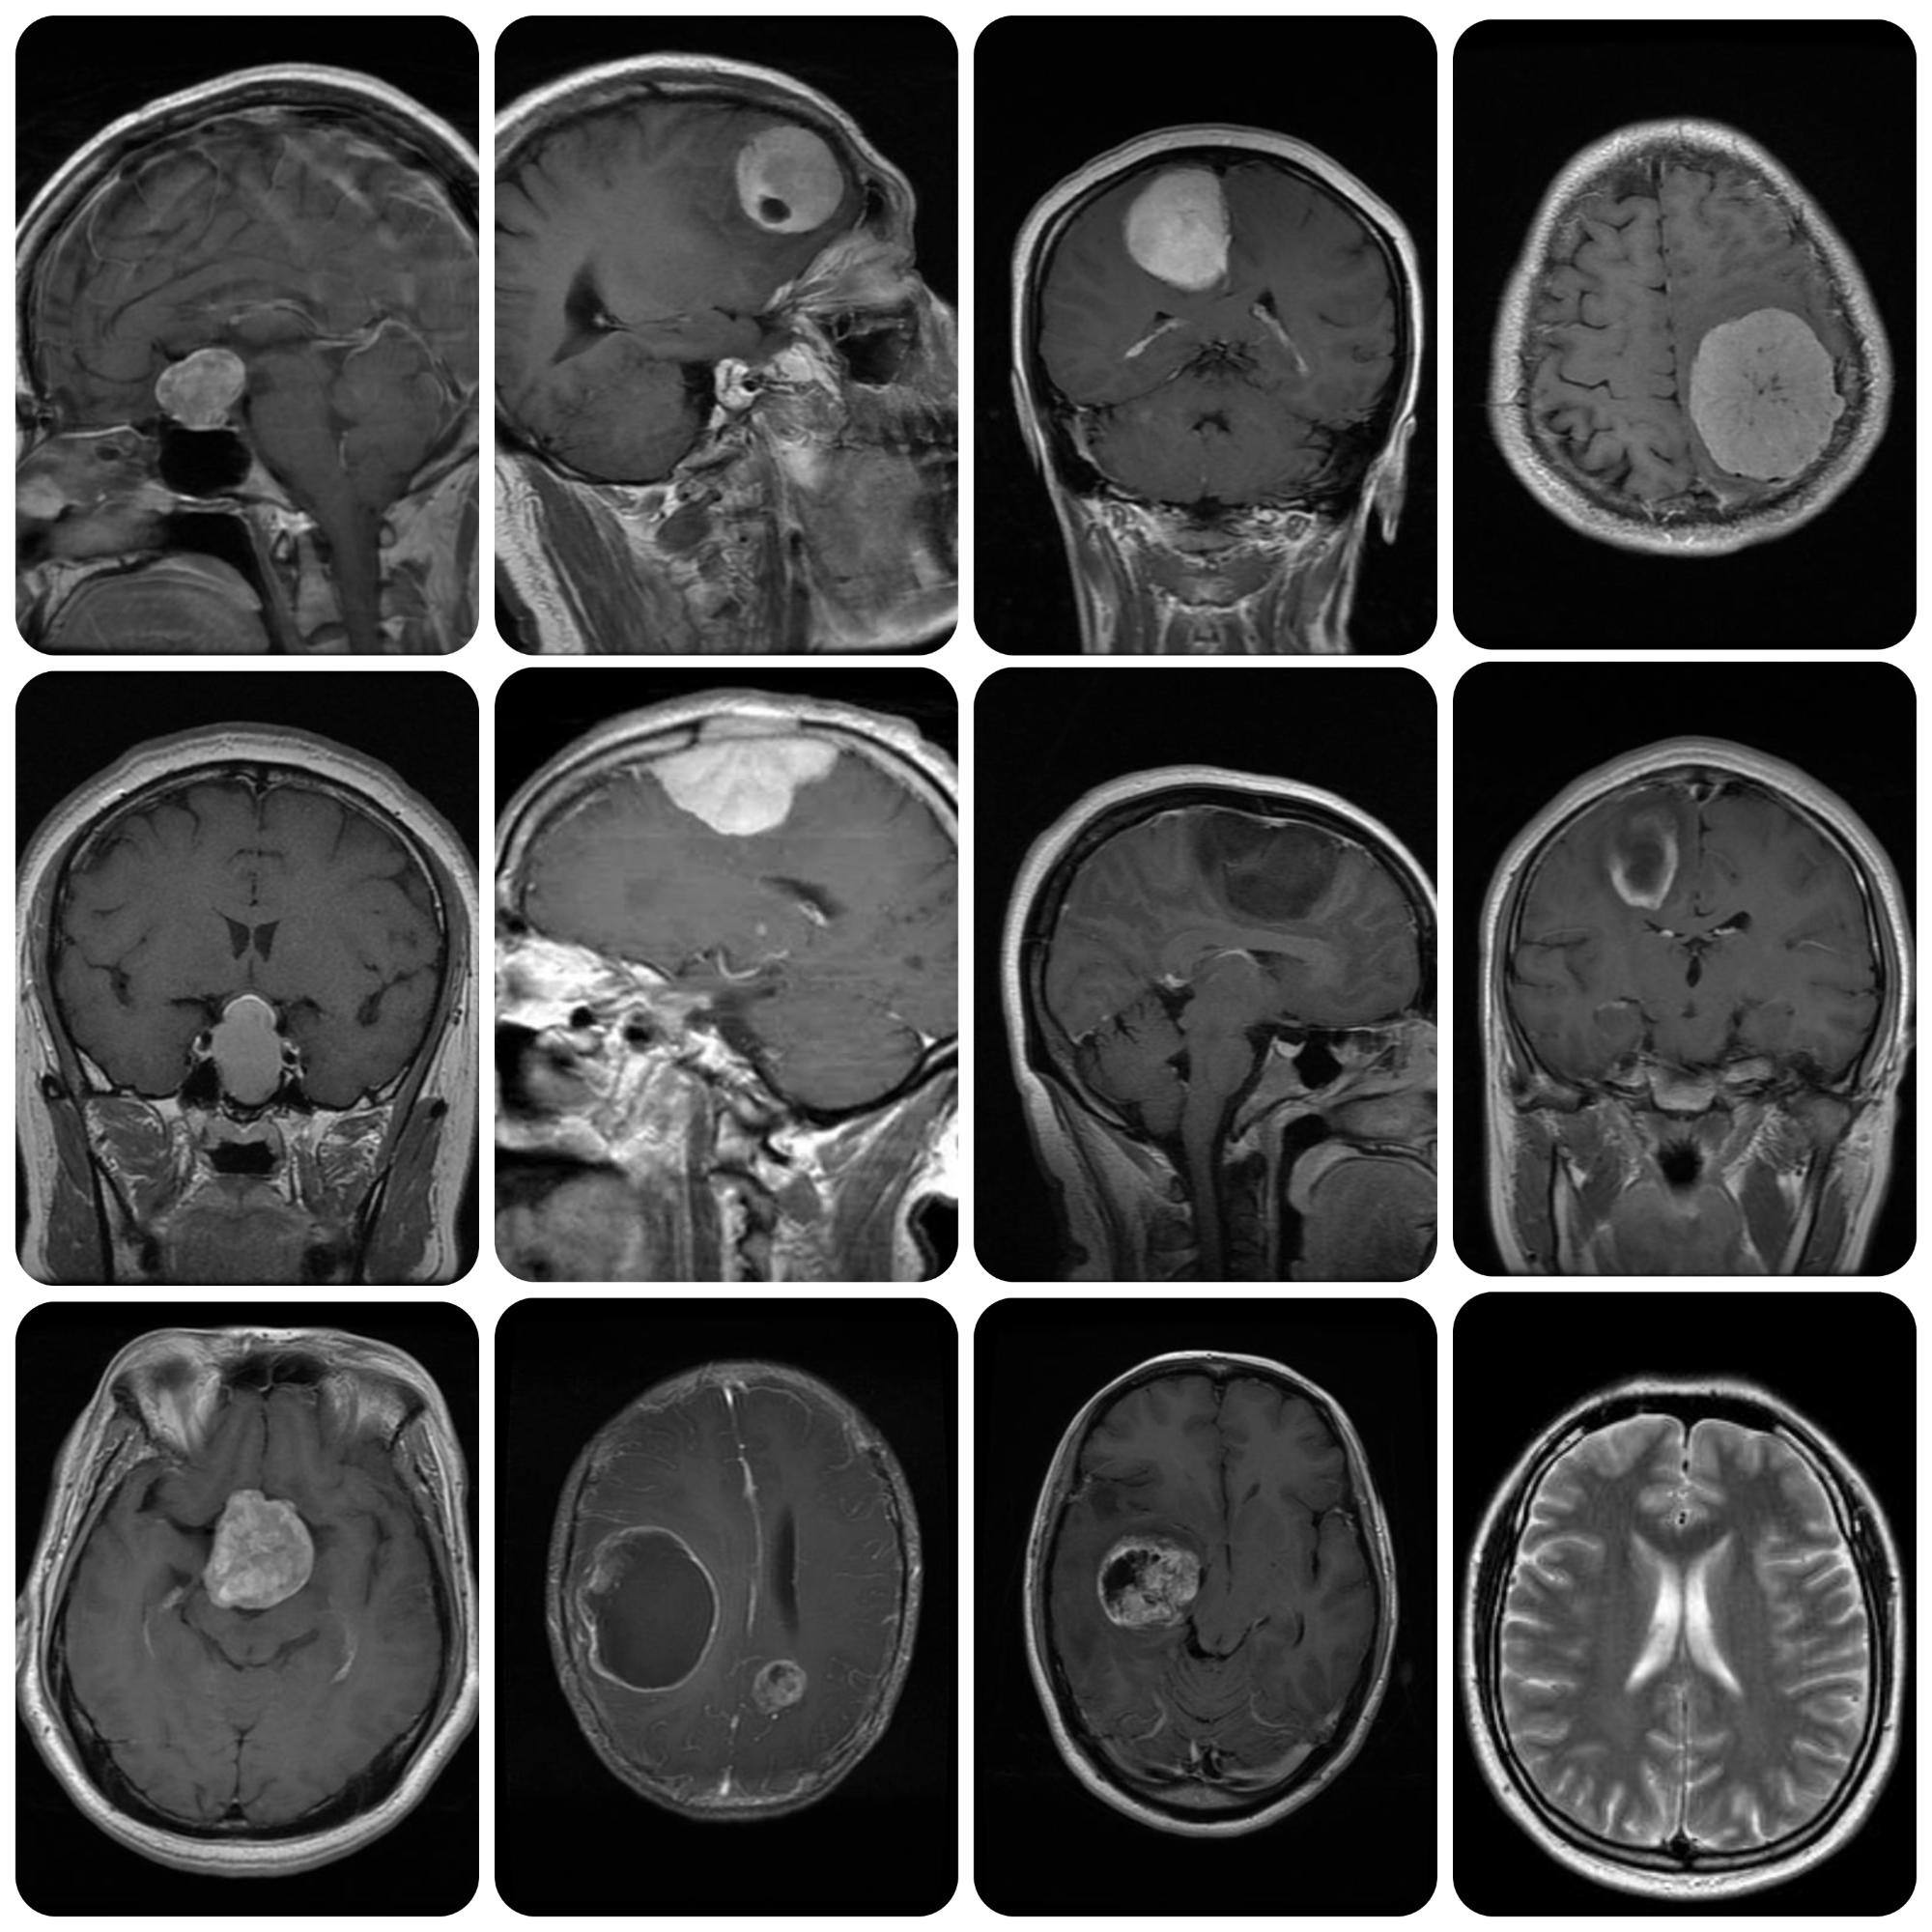
\includegraphics[width=\linewidth]{img/Blank 12 Grids Collage.png}
    \end{subfigure}
    
    \begin{subfigure}{0.9\textwidth}
        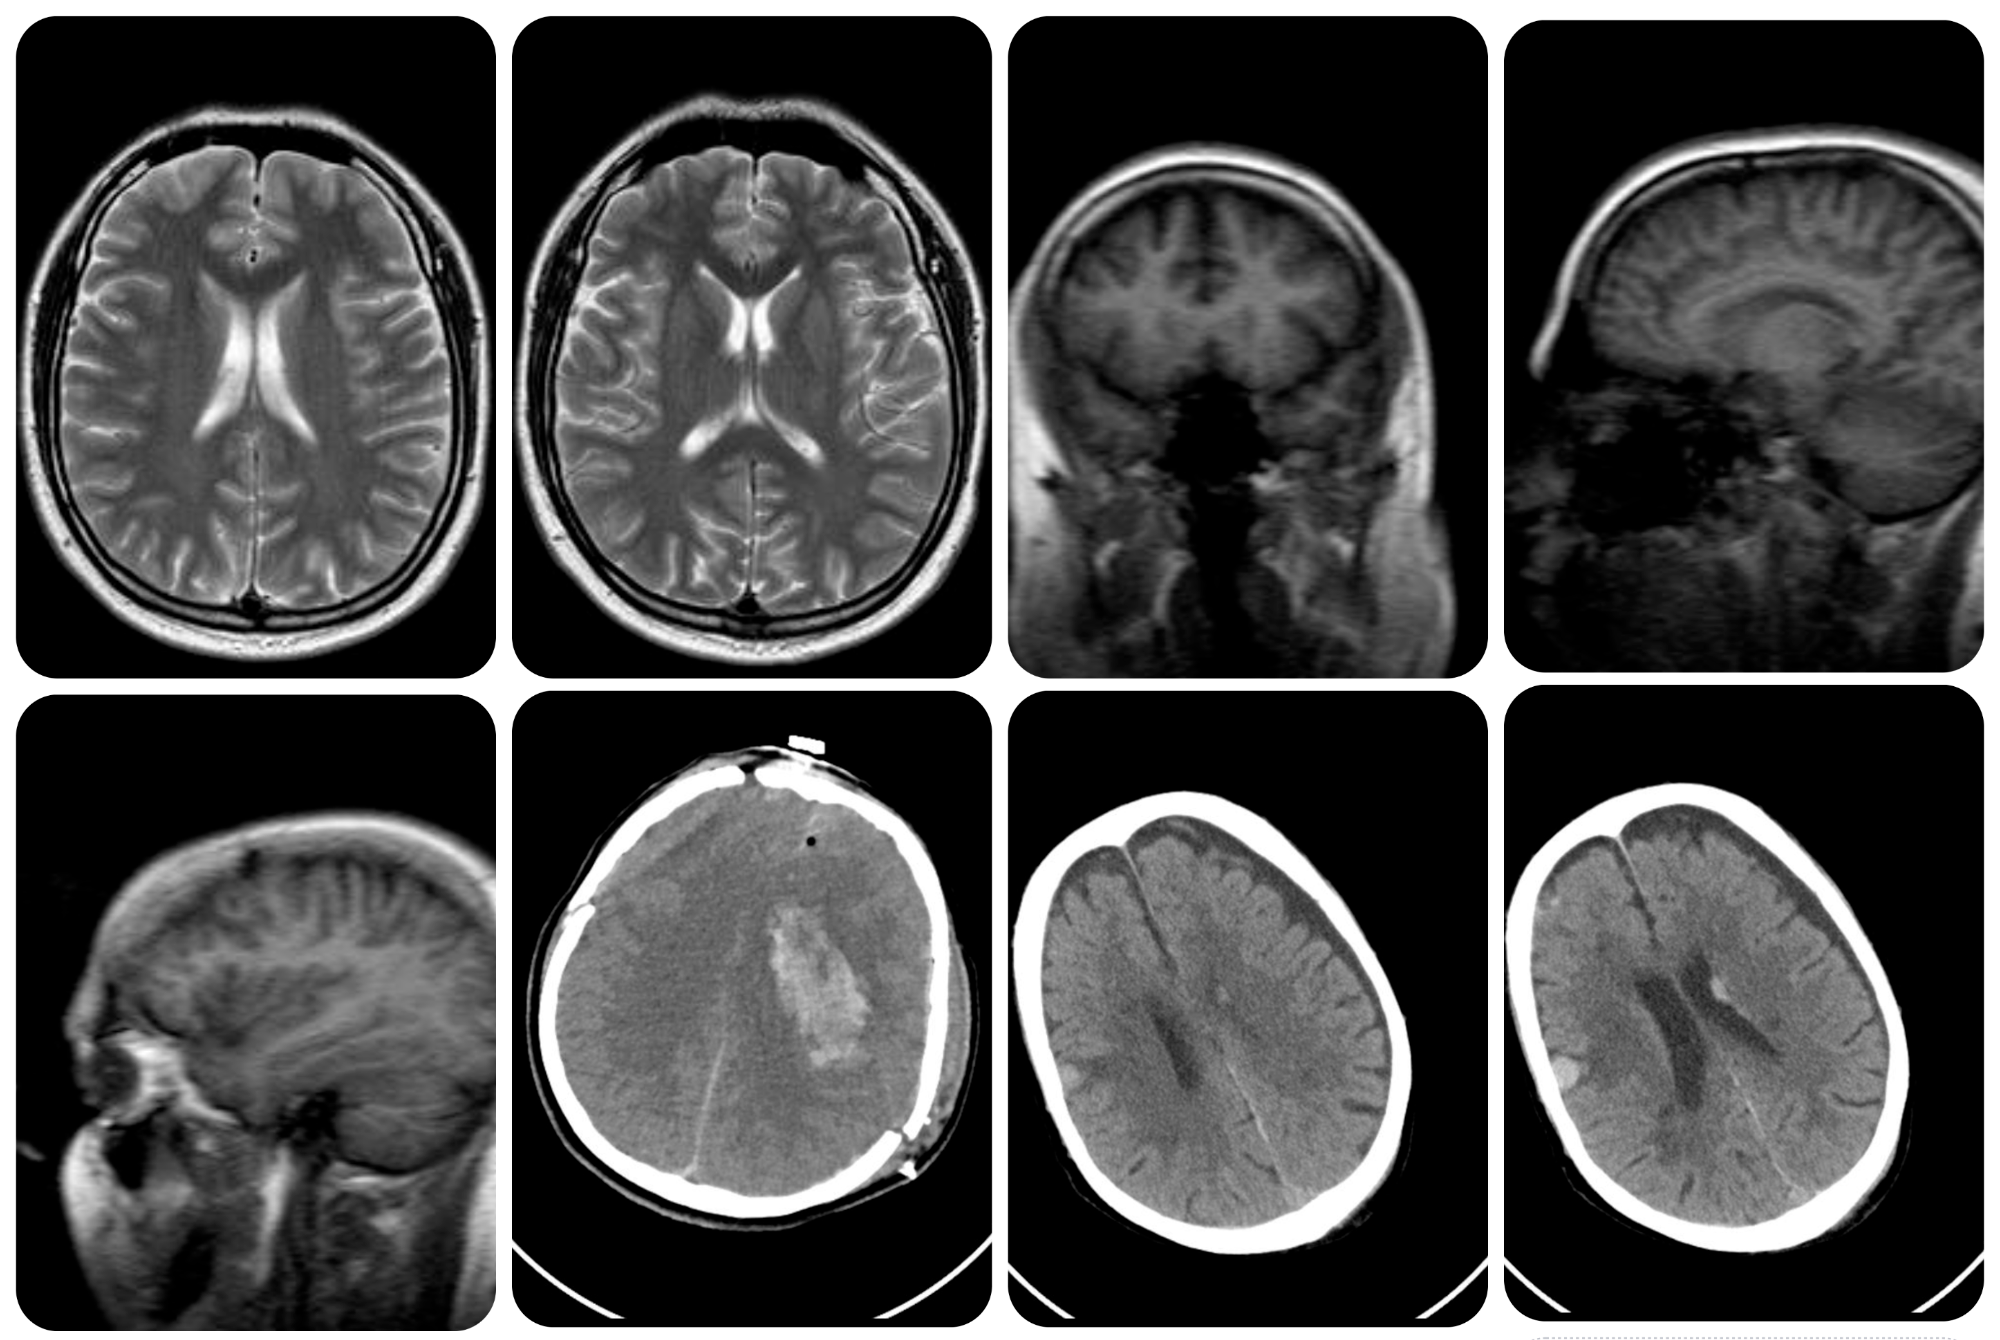
\includegraphics[width=\linewidth]{img/Blank 12 Grids Collage (1).png}
    \end{subfigure}
    \caption{Test images used in the experiments.}
\label{fig:imagenes}    
\end{figure}

\noindent The experimental design is multifactorial, focusing on three main factors: the evaluation of the fitness function, the signal-to-noise ratio (PSNR), and the Structural Similarity Index (SSIM). Eight different treatments corresponding to the selected algorithms were carried out: Reptile Search (RSA)~\cite{Abualigah2022}, Orca Predator (OPA)~\cite{Jiang2022}, Honey Badger Algorithm (HBA)~\cite{Hashim2022}, Bald Eagle Search (BES)~\cite{Alsattar2019}, Gray Wolf Optimization (GWO)~\cite{Mirjalili2014}, Crow Search (CSA)~\cite{Askarzadeh2016}, Harris Hawk Optimization (HHO)~\cite{Heidari2019}, and Tuna Swarm Optimization (TSO)~\cite{Xie2021}. The parameters used were tabulated in Table~\ref{tab:algorithms-parameters}, with a population of 30, a set iteration of 100, and 30 independent runs were conducted for each algorithm.

\begin{table}[!t]
	\renewcommand{\arraystretch}{1.3}
	\caption{Algorithms and parameters}
	\label{tab:algorithms-parameters}
	\centering
	\begin{tabular}{|c|c|}
		\hline
		\textbf{Algorithms} & \textbf{parameters} \\
		\hline
		BES                 &                      
		\begin{tabular}{@{}c@{}}
		$c1=c2=2$ \\
		$\alpha=2$ \\
		$a=10$ \\
		$R=1.5$
	\end{tabular} \\
	\hline
	HHO & - \\
	\hline
	OPA &
	\begin{tabular}{@{}c@{}}
		$p1,p2=[0,1]$ \\
		$a=0.01$      
	\end{tabular} \\
	\hline
	CSA &
	\begin{tabular}{@{}c@{}}
		$fl=2$   \\
		$AP=0.1$ 
	\end{tabular} \\
	\hline
	GWO & $a=2$ (linear decreasing) \\
	\hline
	HBA &
	\begin{tabular}{@{}c@{}}
		$\beta=6$ \\
		$C=2$     
	\end{tabular} \\
	\hline
	RSA &
	\begin{tabular}{@{}c@{}}
		$\alpha=0.1$ \\
		$\beta=0.1$  
	\end{tabular} \\
	\hline
	TSO &
	\begin{tabular}{@{}c@{}}
		$z=0.05$ \\
		$a=0.7$  
	\end{tabular} \\
	\hline
	\end{tabular}
\end{table}

\subsection{Activity Description}
\noindent The primary focus of the research was the in-vivo analysis of the brain using medical image sequences from public datasets. Magnetic Resonance Imaging (MRI) and Computed Tomography (CT) images, which included various brain pathologies, were used to study the effectiveness of segmentation processes. The goal was to achieve the most accurate segmentation of cerebral tissue using advanced optimization methods.

\noindent For this purpose, Kapur, Otsu, and Tsallis algorithms, which have been previously validated for their efficacy in segmenting complex anatomical structures in medical images, were applied. These algorithms were tested in our study to determine which provides better results in terms of segmentation accuracy.

\noindent Furthermore, an exhaustive analysis was carried out using a Python script, which implemented these algorithms to evaluate the segmentation thresholds in MRI and CT images. Performance metrics such as the Signal-to-Noise Ratio (PSNR) and the Structural Similarity Index (SSIM) were assessed to ensure the quality and accuracy of the segmentation. Each algorithm was executed multiple times to confirm the robustness of the results obtained.

\noindent This comprehensive approach not only enhanced the understanding of segmentation techniques applied to specific brain pathologies but also optimized the processes of medical image analysis for future research.

\subsubsection{Validity Evaluation}

\noindent To ensure the validity of the results obtained in the experimentation with the bioinspired metaheuristic algorithms, several criteria and procedures were established. The validity of the study is addressed from different dimensions: internal validity, which refers to the accuracy with which the treatments reflect variations in the outcomes; external validity, which evaluates the generalization of the results to other contexts; and construct validity, which verifies that the operationalization truly measures the phenomenon under study.

\subsubsection{Internal Validity}
\noindent For internal validity, extrinsic variables that could influence the performance of the algorithms, such as lighting and quality of the medical images, were controlled. Additionally, the same evaluation protocol was used for all treatments, which includes the optimization function and evaluation indices (PSNR and SSIM). The consistency of the experimental conditions was verified through detailed recording of each step in the algorithm execution procedure.

\subsubsection{Validez Externa}
\noindent Respecto a la validez externa, se seleccionó una muestra de imágenes de sujetos de prueba con múltiples patologías cerebrales para que los hallazgos puedan ser extrapolados a una amplia variedad de casos clínicos. Sin embargo, se reconoce que la investigación podría beneficiarse de estudios adicionales que examinen la aplicabilidad de los algoritmos en escenarios clínicos aún más variados.

\subsubsection{Construct Validity}
\noindent Construct validity was ensured through the use of algorithms whose performance has been corroborated in previous research. To strengthen this validity, the performance metrics used (fitness, PSNR, and SSIM) are widely recognized and employed in the field of medical image processing and analysis.

\noindent To provide a solid foundation for the evaluation of validity, a pretest of the algorithms and a pilot of the experimental design were conducted on a subset of the sample before full implementation. This allowed for the detection and correction of possible flaws in the proposed methodology. Additionally, the replicability of the research is facilitated by the thorough documentation and availability of the source code used, allowing future studies to verify and build upon our findings.
\subsubsection{Conclusion Validity}

\noindent To ensure conclusion validity, the Wilcoxon signed-rank test was applied to our algorithm segmentation comparisons. This non-parametric statistical test is ideal for small samples or data that do not distribute normally. A significance level was set a priori, and the effect size was evaluated to determine the practical relevance of the results. By controlling for Type I and II errors, we ensured the statistical robustness of our conclusions, limiting the possibility of misinterpretations of the treatment effect.

\subsection{Data Analysis Definition}

\noindent In the data analysis phase of our study, the main statistical approach employed will be the Friedman test. This non-parametric test will be used to evaluate differences in performance metrics —fitness, Structural Similarity (SSIM), and Signal-to-Noise Ratio (PSNR)— among the various segmentation algorithms applied to the dataset of medical images.

\noindent Each metric will be analyzed independently using this test to identify if the improvements obtained by the different algorithms are statistically significant. Statistical significance will be established with a predefined p-value. Additionally, the effect size will be calculated for each comparison to quantify the magnitude of the observed differences.

\noindent Upon concluding the analysis, the results will provide a detailed perspective on the relative performance of each algorithm, facilitating the identification of the most effective methods for in-vivo brain segmentation.

%----------------------------------


%-----------------------------------
\section{Metaheuristic Algorithms}
\noindent In this section, multilevel thresholding is performed using metaheuristic algorithms by maximizing Kapur's entropy ~\ref{eq_Kapur}, Otsu's method ~\ref{eq_Otsu}, and Tsallis's entropy ~\ref{eq_Tsallis} as follows:
\begin{equation}
\begin{gathered}
\max(F_{kapur}(th)) \
\text{th} \in 0 \leq \text{th}_i \leq 255
\end{gathered}
\label{eq_Kapur}
\end{equation}
\noindent where $i=[1,2,...,n]$, with $n$ being the number of thresholds.
\begin{equation}
\begin{gathered}
\max(\sigma_B^2(th)) \
\text{th} \in 0 \leq \text{th} \leq 255
\end{gathered}
\label{eq_Otsu}
\end{equation}
\begin{equation}
\begin{gathered}
\max(J_{Tsallis}(\mathbf{t})) \
\mathbf{t} = (t_1, t_2, \dots, t_k) \in \mathbb{Z}^k \
0 \leq t_i \leq 255, \quad i = 1, 2, \dots, k
\end{gathered}
\label{eq_Tsallis}
\end{equation}
\noindent where $J_{Tsallis}(\mathbf{t})$ is the Tsallis entropy for a given threshold vector $\mathbf{t}$, defined as:
\begin{equation}
J_{Tsallis}(\mathbf{t}) = \sum_{i=1}^{k+1} \frac{w_i}{w_T} S_i + (1-q) \prod_{i=1}^{k+1} S_i
\end{equation}
\noindent with $S_i$ being the Tsallis entropy for region $i$:
\begin{equation}
S_i = \frac{1}{q-1}\left(1 - \sum_{p=l_i}^{u_i} \left(\frac{h(p)}{w_i}\right)^q\right)
\end{equation}
\noindent and $q$ is the non-extensivity parameter, $l_i$ and $u_i$ are the lower and upper limits of region $i$, $w_i$ is the weight of region $i$, $h(p)$ is the normalized histogram for pixel value $p$, and $w_T$ is the total weight of the image.
The metaheuristic algorithms aim to find the optimal threshold vector $\mathbf{t}^*$ that maximizes the Tsallis entropy:
\begin{equation}
\mathbf{t}^* = \arg\max_{\mathbf{t}} J_{Tsallis}(\mathbf{t})
\end{equation}

\noindent Here, $\sigma_B^2(th)$ represents the between-class variance for a threshold $th$, and the objective is to find the value of $th$ that maximizes this variance, with $th$ varying in the range of 0 to 255 for 8-bit grayscale images.

\subsection{Bald Eagle Search}

\noindent The Bald Eagle Search (BES) algorithm, proposed by Alsattar et al.~\cite{Alsattar2019}, is a bio-inspired metaheuristic algorithm that mimics the hunting strategy or intelligent social behavior of bald eagles while hunting fish.

\noindent The area identification stage relates to the bald eagle when it performs a search for the best position $P$ to hunt for food (select space). This stage is mathematically represented as:

\begin{equation}
\begin{gathered}
P_{new}=P_{best}+{\alpha}r(P_{mean}-P_{i})\\
\end{gathered}
\label{eq11}
\end{equation}

\noindent Once the best position in space is selected, the bald eagle performs different spiral movements to increase the speed of the food search process. This stage is called search within the area (search space) and is mathematically represented as:

\begin{equation}
\begin{gathered}
P_{new}=P_{i}+y(i)(P_{i}-P_{i+1})+x(i)(P_{i}-P_{mean}) \\
x(i)= \frac{xr_{i}}{max(\lvert xr \rvert)} ~\ , ~\ y(i)= \frac{yr_{i}}{max(\lvert yr \rvert)} \\
xr(i)=r(i)\cdot \sin (\theta(i)) ~\ , ~\ yr(i)=r(i)\cdot \cos (\theta(i)) \\
\theta(i)=a\cdot r\cdot rnd ~\ , ~\ r(i)=\theta(i)+R \cdot rnd 
\end{gathered}
\label{eq12}
\end{equation}

\noindent The last stage of the BES algorithm corresponds to the selection and attack of the prey, called swoop. The swoop consists of moving all the best points towards the target. Mathematically, this is expressed as:

\begin{equation}
\begin{gathered}
P_{\text{new}} = \text{rnd} \cdot P_{\text{best}} + x1(i)(P_{i}-c1 \cdot P_{\text{mean}}) \\
+ y1(i)(P_{i}-c2 \cdot P_{\text{best}}) \\
x1(i) = \frac{xr_{i}}{\max(\lvert xr \rvert)}, \quad y1(i) = \frac{yr_{i}}{\max(\lvert yr \rvert)} \\
xr(i) = r(i) \cdot \sinh(\theta(i)), \quad yr(i) = r(i) \cdot \cosh(\theta(i))
\end{gathered}
\end{equation}

\subsection{Harris Hawk Optimization}

\noindent The Harris Hawk Optimization (HHO) algorithm is a bio-inspired algorithm proposed by Heidari et al.~\cite{Heidari2019} based on the behavior of Harris Hawks. The algorithm was modeled through the exploration and exploitation phases. In the exploration phase, the Harris Hawk can detect and track its prey with its powerful eyes. In HHO, the Harris Hawk can randomly stay in some locations and wait to detect prey based on its strategy. If an equal chance $q$ is considered for each perched strategy based on the position of family members, it can be modeled as a condition $q<0.5$, or perched at a random position in the trees as $q\geq 0.5$, as shown:

\begin{equation}
\begin{gathered}
X(t+1)= \\
\begin{cases}
  X_{rnd}(t) - r_1 |X_{rnd}(t) -2 r_2 X(t)| , q \geq 0.5 \\
  X_{rab}(t) - X_m(t) - r3(LB + r_4 (UB-LB)) , q < 0.5
\end{cases}
\end{gathered}
\end{equation}

\noindent The average position can be calculated by:
\begin{equation}
X_m (t) = \frac{1}{N} \sum_{i=1}^{N} X_i(t) 
\label{eq14}
\end{equation}

\noindent In the transition from exploration to exploitation, when prey escapes, it loses energy. This loss is modeled as:
\begin{equation}
E = 2 E_0 (1 - \frac{t}{T}) 
\label{eq15}
\end{equation}

\noindent The parameter $E$ indicates the escape energy of the prey, and $T$ is the maximum number of iterations. On the other hand, $E_0$ is a random parameter that oscillates between $(-1,1)$ for each iteration.

\noindent The exploitation phase is divided into soft besiege and hard besiege. In soft besiege, the conditions $r \geq 0.5$ and $|E| \geq 0.5$ must be met. The prey tries to escape through some random jumps but finally fails. This is modeled as:

\begin{equation}
\begin{gathered}
X(t+1) = \Delta X(t) - E |J X_{rabb}(t) -X(t)| \\
\Delta X(t) = X_{rabb}(t) - X(t)
\end{gathered}
\label{eq16}
\end{equation}

\noindent In hard besiege, $r \geq 0.5$ and $|E| < 0.5$ must be met. The prey is tired to escape. In this case, the position is updated according to:

\begin{equation}
\begin{gathered}
X(t+1) = X_{rabb}(t) - E |\Delta X(t)| \\
\end{gathered}
\label{eq17}
\end{equation}

\subsection{Orca Predator Algorithm}

\noindent The Orca Predator Algorithm (OPA), proposed by Jiang et al.~\cite{Jiang2022}, is a metaheuristic algorithm bio-inspired by the behavior of Orcas. Orcas are highly intelligent carnivorous beings in the dolphin family. They live in families with approximately 30 members. Orcas communicate with each other through sounds, coordinating their movements to herd fish, drive them to the surface, and finally encircle them. The Orca group model can swim in $1-D, 2-D, 3-D$ or in an extra-dimensional space. This is defined as:

\begin{equation}
\begin{gathered}
X = [ x1, x2, ..., xN ] =\begin{bmatrix}
  x1,1 & x1,2 & ... & x1,D  \\
  x2,2 & x2,2 & ... & x2,D  \\
  \vdots & \vdots & \vdots & \vdots \\
  xN,1 & xN,2 & ... & xN,D
\end{bmatrix}
\end{gathered}
\label{eq18}
\end{equation}

\noindent The movement of Orcas herding fish can be modeled by the movement velocity as follows:

\begin{equation}
\begin{gathered}
v_{chase,1,i}^t = a ( d x_{best}^t - F (b M^t + c x_i^t)) \\
v_{chase,2,i}^t = e x_{best}^t - x_{i}^t \\
M = \frac{\sum_{i=1}^{N} x_i^t}{N} \\
c=1-b \\
\begin{cases}
  x_{chase,1,i}^t = x_{i}^t + v_{chase,1,i}^t , \text{if} \;rand > q \\
  x_{chase,2,i}^t = x_{i}^t + v_{chase,2,i}^t  , \text{if} \;rand \leq q
\end{cases}
\end{gathered}
\label{eq19}
\end{equation}

\noindent The herding of prey is performed by the position of three randomly selected Orcas, and then their position can be determined as:
\begin{equation}
\begin{gathered}
x_{chase,3,i}^t =x_{j1,k}^t +u \times (x_{j2,k}^t - x_{j3,k}^t ) \\
u = 2 \times (\text{rand} - \frac{1}{2}) \times \frac{Max_{iter}-t}{Max_{iter}}
\end{gathered}
\label{eq20}
\end{equation}

\noindent The position adjustment is determined by comparing the best values obtained in the fitness function, modeled as:

\begin{equation}
\begin{gathered}
\begin{cases}
  x_{chase,i}^t = x_{chase,i}^t \;\;, \text{if} \; f(x_{chase,i}^t) < f(x_{i}^t ) \\
  x_{chase,t}^t = x_{i}^t  \;\;, \text{if} \;f(x_{chase,i}^t) \geq f(x_{i}^t )
\end{cases}
\end{gathered}
\label{eq21}
\end{equation}

where $f(x_{chase,i}^t)$ corresponds to the value of the fitness function at $x_{chase,i}^t$, and $f(x_{i}^t )$ corresponds to the value of the fitness function at $x_{i}^t$.

\subsection{Crow Search Algorithm}

\noindent The Crow Search Algorithm (CSA), originally proposed by Askarzadeh et al.~\cite{Askarzadeh2016}, is a metaheuristic algorithm bio-inspired by the behavior of Crows. Crows are considered the most intelligent birds. They observe other birds, noting where they hide their food, and steal it when they are not around. In fact, they use their own experience of having been thieves to predict the behavior of a thief and can determine the safest path to protect their treasures against theft. The first step is associated with position and is modeled as:

\begin{equation}
\begin{gathered}
x^{i,iter} = [x_{1}^{i,iter}, x_{2}^{i,iter},...,x_{d}^{i,iter}]\\
x^{i,iter+1}=x^{i,iter}+r_{i} \times fl^{i,iter} \times (m^{j,iter}-x^{i,iter})
\end{gathered}
\label{eq23}
\end{equation}

\noindent Crow $j$ knows that crow $i$ is following it. As a result, to protect its cache against theft, crow $j$ deceives crow $i$ by going to another position in the search space. This is modeled as:

\begin{equation}
\begin{gathered}
x^{i,iter+1}=\\
\begin{cases}
x^{i,iter}+r_{i} fl^{i,iter} (m^{j,iter} - x^{i,iter}) \; \; \; r_j \geq AP^{i,iter}\\
\text{a random position} \; \; \; \; \; \;\; \; \;\; \; \;\;\; \; \;\;\; \; \; \; \;\;\; \; \;\; \; \;  \text{otherwise}
\end{cases}
\end{gathered}
\label{eq24}
\end{equation}

\subsection{Gray Wolf Optimization}

\noindent The Gray Wolf Optimization (GWO) algorithm, originally proposed by Mirjalili et al.~\cite{Mirjalili2014}, is a metaheuristic algorithm bio-inspired by the behavior of Gray Wolves. Gray Wolves are considered super predators, living in packs with group sizes ranging from 5 to 12 individuals. Mathematically, a hierarchy within the pack is considered, where the values of the solutions are stored in order, in $\alpha$, $\beta$, and $\delta$, as first, second, and third, respectively. The remaining solutions are stored in $\omega$. The GWO algorithm stores the hunt guided by $\alpha,\beta$ and $\delta$ while $\omega$ follows the other variables.

\noindent The hunting phase begins with encircling the prey, modeled as:

\begin{equation}
\begin{gathered}
\vec{D} = |\vec{C} \times \vec{X_p}(t)-\vec{X}(t)|\\
\vec{X}(t+1) = \vec{X_p}(t) - \vec{A} \times \vec{D}
\end{gathered}
\label{eq25}
\end{equation}

\noindent where $\vec{A}$ and $\vec{C}$ are vector coefficients, and $\vec{X}$ is the position. The hunt is guided by the alpha, while beta and delta do not usually participate. Mathematically, it is assumed that alpha, beta, and delta have the best knowledge about the position of the prey. Then, the three best solutions are stored, and the other agents are forced to move and update their positions according to the best solutions.

\begin{equation}
\begin{gathered}
\vec{D}_{\alpha} = |\vec{C}_1 \times \vec{X}_{\alpha} -\vec{X}|, \vec{D}_{\beta} = |\vec{C}_1 \times \vec{X}_{\beta} -\vec{X}| \\
\vec{D}_{\delta} = |\vec{C}_1 \times \vec{X}_{\delta} -\vec{X}|\\
\vec{X}_1=\vec{D}_{\alpha}-\vec{A}_1 \times (\vec{D}_{\alpha}), \vec{X}_2=\vec{D}_{\beta}-\vec{A}_2 \times (\vec{D}_{\beta})\\
\vec{X}_3=\vec{D}_{\delta}-\vec{A}_3 \times (\vec{D}_{\delta}) \\
\vec{X}(t+1) = \frac{\vec{X}_1+\vec{X}_2+\vec{X}_3}{3}
\end{gathered}
\label{eq26}
\end{equation}
\subsection{Honey Badger Algorithm}

\noindent The Honey Badger Algorithm (HBA), originally proposed by Hashim et al.~\cite{Hashim2022}, is a bioinspired metaheuristic algorithm based on the behavior of the honey badger. The honey badger follows the honey guide bird, and can also smell and dig at locations where honey is present. The honey guide bird lacks the ability to dig for honey, whereas the honey badger can dig, and it is common for both the honey guide bird and the honey badger to share the reward. The population of candidate solutions is modeled as:

\begin{equation}
\begin{gathered}
\text{Population of candidate solutions}=\\\begin{bmatrix}
  x1,1 & x1,2 & ... & x1,D  \\
  x2,2 & x2,2 & ... & x2,D  \\
  \vdots & \vdots & \vdots & \vdots \\
  xn,1 & xn,2 & ... & xn,D
\end{bmatrix}
\end{gathered}
\label{eq27}
\end{equation}

\noindent The intensity is related to the concentration power of the prey and the distance between the prey and the $ith$ honey badger. The intensity of the prey's scent is represented by $I_i$, where a high scent intensity leads to faster movement and vice versa. This is defined as:

\begin{equation}
\begin{gathered}
I_1 = r_2 \times \frac{S}{4 \pi d_i^2}\\
S = (x_i - x_{i+1})^2\\
d_i = x_{prey} - x_i
\end{gathered}
\label{eq28}
\end{equation}

\noindent $S$ represents the concentration power, $d_i$ denotes the distance between the prey and the $ith$ honey badger. Additionally, the density factor $\alpha$ controls the randomization of the time-variant to ensure a transition from exploration to exploitation, as shown:

\begin{equation}
\begin{gathered}
\alpha = C \times exp\left(-\frac{t}{t_{max}}\right)\\
\end{gathered}
\label{eq29}
\end{equation}

\noindent In the digging phase, the honey badger performs a cardioid movement, as follows:

\begin{equation}
\begin{gathered}
x_{new} = x_{prey} + F \times \beta \times I \times x_{prey} + \\
F \times r_3 \times \alpha \times d_i \times \left|\cos(2\pi r_4) \times [1-\cos(2\pi r_5)]\right|
\end{gathered}
\label{eq30}
\end{equation}

\noindent $x_{prey}$ corresponds to the position of the prey, $r_3$, $r_4$, and $r_5$ are random numbers between 0 and 1. $F$ acts as a flag that alters the search direction, as follows:

\begin{equation}
\begin{gathered}
F=
\begin{cases}
1, & \text{if } r_6 \leq 0.5 \\
-1, & \text{otherwise}
\end{cases}
\end{gathered}
\label{eq31}
\end{equation}    

\noindent $r_6$ is a random number between 0 and 1. Finally, the position is updated by the honey guide bird, which can be simulated as:

\begin{equation}
\begin{gathered}
x_{new} = x_{prey} + F \times r_7 \times \alpha \times d_i
\end{gathered}
\label{eq32}
\end{equation}

\noindent $r_7$ is a random number between 0 and 1.

\subsection{Reptile Search Algorithm}

\noindent The Reptile Search Algorithm (RSA), originally proposed by Abualigah et al.~\cite{Abualigah2022}, is based on the behavior of crocodiles during hunting. 
\noindent Equation 1 is generated stochastically, and the best solution is considered closest to the optimum in each iteration.

\begin{equation}
\begin{gathered}
X = \begin{bmatrix}
  x1,1 & x1,2 & ... & x1,n  \\
  x2,2 & x2,2 & ... & x2,n  \\
  \vdots & \vdots & \vdots & \vdots \\
  xN,1 & xN,2 & ... & xN,n
\end{bmatrix}
\end{gathered}
\label{eq33}
\end{equation}

\noindent The exploration phase is defined by:

\begin{equation}
\begin{gathered}
x_{(i,j)}(t+1)=\\
\begin{cases}
Best_j (t) - \eta_{(i,j)} \times \beta - R_{(i,j)}(t) \times rand, & t \leq \frac{T}{4} \\
Best_j (t) \times x_{(r_1,j)} \times ES(t) \times rand, & t \leq 2\frac{T}{4} and t \geq \frac{T}{4} \\
\end{cases}
\end{gathered}
\label{eq34}
\end{equation}   

\begin{equation}
\begin{gathered}
\eta_{(i,j)} = Best_j(t) \times P_{(i,j)}
\end{gathered}
\label{eq35}
\end{equation}

\begin{equation}
\begin{gathered}
R_{(i,j)} = \frac{Best_j(t) - x_{(r_2,j)}}{Best_j(t) + \epsilon}
\end{gathered}
\label{eq36}
\end{equation}

\begin{equation}
\begin{gathered}
ES(t) = 2 \times r_3 \times (1 - \frac{1}{T})
\end{gathered}
\label{eq37}
\end{equation}

\begin{equation}
\begin{gathered}
P_{(i,j)} = \alpha + \frac{x_{(i,j) - M(x_i)}}{Best_j(t) \times (UB_{(j)}-LB_{(j)}) + \epsilon} 
\end{gathered}
\label{eq38}
\end{equation}

\begin{equation}
\begin{gathered}
M_{(x_i)} = \frac{1}{n} \sum_{j=1}^{n} x_{(i,j)}
\end{gathered}
\label{eq39}
\end{equation}
\subsection{Tuna Swarm Optimization}

\noindent The Tuna Swarm Optimization (TSO), proposed by Xie et al.~\cite{Xie2021}, is inspired by the foraging strategies of tunas, which include spiral and parabolic formations for hunting prey.

\subsubsection{Initialization}

\noindent The initialization of TSO is performed by generating initial populations randomly and uniformly within the search space:
\begin{equation}
    \begin{gathered}
        X_{\text{init}} = \\
        \text{rand} \cdot (ub - lb) + lb, \quad i = 1, 2, ..., NP
    \end{gathered}
\end{equation}

\noindent where $X_{\text{init}}$ is the $i$-th initial individual, $ub$ and $lb$ are the upper and lower bounds of the search space, $NP$ is the number of tuna populations, and $\text{rand}$ is a uniformly distributed random vector from 0 to 1.

\subsubsection{Spiral Foraging}
Spiral foraging is modeled as follows, adjusting the position of tunas towards an optimum point or a random reference point based on the phase of the iteration:
\begin{equation}
    \begin{gathered}
        X_{t+1}^i = \\
        \quad
        \begin{cases}
            \alpha_1 \cdot \left(X_{\text{best}}^t + \beta \cdot \left\lVert X_{\text{best}}^t - X_t^i \right\rVert \right) + \alpha_2 \cdot X_t^i, & \text{if } i = 1,\\
            \alpha_1 \cdot \left(X_{\text{rand}} + \beta \cdot \left\lVert X_{\text{rand}} - X_t^i \right\rVert \right) + \alpha_2 \cdot X_t^{i-1}, & \text{if } i = 2,3,...,NP,
        \end{cases}
    \end{gathered}
\end{equation}

where $\alpha_1$, $\alpha_2$ are weighting coefficients, $\beta$ involves a random variable $b$, and $X_{\text{rand}}$ is a random reference point.

\subsubsection{Parabolic Foraging}
Parabolic foraging is described as:
\begin{equation}
    \begin{gathered}
        X_{t+1}^i = \\
        \begin{cases}
            X_{\text{best}}^t + \text{rand} \cdot (X_{\text{best}}^t - X_t^i) + TF \cdot p^2 \cdot (X_{\text{best}}^t - X_t^i), & \text{if rand } < 0.5,\\
            TF \cdot p^2 \cdot X_t^i, & \text{if rand } \geq 0.5,
        \end{cases}
    \end{gathered}
\end{equation}

\noindent where $TF$ is a random number with a value of 1 or -1, and $p$ is a probability that varies with the iteration.

\noindent These strategies enable TSO to perform effective global exploration and precise local exploitation of the search space. Individuals in the algorithm alternate between spiral and parabolic foraging strategies, adapting their behavior to find optimal solutions.

\section{Results Analysis}
\subsection{Metrica Fitness}
\noindent En las evaluaciones realizadas con las funciones objetivo de Kapur, Otsu y Tsallis, se observa un patrón consistente ~\ref{sec:appendix} en el rendimiento de los algoritmos a través de las dimensiones 7, 8 y 9:
\begin{itemize}
    \item \textbf{GWO y TSO} se destacan como los algoritmos más efectivos, mostrando el mejor rendimiento general en todas las funciones objetivo.
    \item \textbf{HBA y OPA} generalmente ofrecen buenos resultados, ubicándose después de GWO y TSO en términos de efectividad.
    \item \textbf{RSA y BES} muestra consistentemente el peor desempeño en todas las pruebas realizadas.
\end{itemize}

\subsection{Test de Friedman, Metrica SSIM}
\subsubsection{Función objetivo Kapur}
\noindent En el análisis~\ref{fig:SSIM_Kapur_Friedmann} mediante el test de Friedman para la función objetivo de Kapur y la métrica SSIM. Los resultados revelaron que GWO fue consistentemente el algoritmo más destacado, con rankings promedio entre 1.3 y 2.1, seguido de HBA con rankings entre 2.15 y 3.05. OPA, CSA y HHO mostraron un desempeño intermedio, mientras que RSA, BES y TSO registraron los rankings más bajos. Este patrón se mantuvo constante en todas las dimensiones evaluadas, indicando una clara jerarquía de eficacia entre los algoritmos.

\begin{figure}[H]
    \centering
    
\includegraphics[width=0.8\textwidth]{SSIM/Kapur/Metrica_kapur_Friedman_results.png}
    \caption{Average Rank of the SSIM metric by dimension K, Kapur entropy objective function}
    \label{fig:SSIM_Kapur_Friedmann}
\end{figure}

\subsubsection{Función objetivo Otsu}

\noindent Evaluando~\ref{fig:SSIM_Otsu_Friedmann} la métrica SSIM en las dimensiones 7, 8 y 9. Los algoritmos analizados OPA lideró con los rankings más altos, variando de 2.3 a 2.7. GWO también exhibió un rendimiento robusto, con rankings de 2.45 a 3.05. HBA y CSA se ubicaron en posiciones intermedios. OPA se destacó como el algoritmo más efectivo para la función objetivo de Otsu según la métrica SSIM, seguido por GWO, mientras que RSA, BES, HHO y TSO presentaron los peores resultados en las dimensiones evaluadas.

\begin{figure}[H]
    \centering
    
\includegraphics[width=0.8\textwidth]{SSIM/Otsu/Metrica_Otsu_Friedman_results.png}
    \caption{Average Rank of the SSIM metric by dimension K, Otsu objective function}
    \label{fig:SSIM_Otsu_Friedmann}
\end{figure}

\subsubsection{Función objetivo Tsallis}
\noindent Según los resultados~\ref{fig:SSIM_Tsallis_Friedmann} del test de Friedman para la función objetivo de Tsallis y la métrica SSIM en las dimensiones 7, 8 y 9, se observaron diferencias significativas, se destacó CSA consistentemente como el mejor rankings promedio, oscilando entre 1.15 y 1.35, seguido de cerca por GWO, que mantuvo rankings entre 3.0 y 3.2. HBA y OPA se posicionaron en términos intermedios. CSA mostró el mejor desempeño para la función objetivo de Tsallis según la métrica SSIM en todas las dimensiones evaluadas, seguido por GWO, mientras que RSA, BES, HHO y TSO registraron los peores resultados.

\begin{figure}[H]
    \centering
    
\includegraphics[width=0.8\textwidth]{SSIM/Tsallis/Metrica_Tsallis_Friedman_results.png}
    \caption{Average Rank of the SSIM metric by dimension K, Tsallis objective function}
    \label{fig:SSIM_Tsallis_Friedmann}
\end{figure}


\subsection{Test de Friedman, Metrica PSNR}

\subsubsection{Función objetivo Kapur}
\noindent El análisis de los resultados~\ref{fig:PSNR_Kapur_Friedmann} de la prueba de Friedman-Kapur muestra que el algoritmo OPA obtiene consistentemente el mejor rango promedio, con un valor de 2.2, en comparación con los demás algoritmos evaluados en las distintas dimensiones K, BES y TSO se mantiene constante como el peor desempeño a través de las dimensiones evaluadas, desde 7.2 hasta 7.8.

\begin{figure}[H]
    \centering
    
\includegraphics[width=0.8\textwidth]{PSNR/Kapur/Metrica_kapur_Friedman_results.png}
    \caption{Average Rank of the PSNR metric by dimension K, Kapur entropy objective function}
    \label{fig:PSNR_Kapur_Friedmann}
\end{figure}

\subsubsection{Función objetivo Otsu}
\noindent Los resultados~\ref{fig:PSNR_Otsu_Friedmann}, se observa que el algoritmo \textit{OPA} mostró el mejor desempeño, seguido por \textit{RSA}. Los algoritmos \textit{BES}, \textit{TSO}, obtuvieron consistentemente los rangos más altos, indicando un peor desempeño a través de las distintas dimensiones.
\begin{figure}[H]
    \centering
    
\includegraphics[width=0.8\textwidth]{PSNR/Otsu/Metrica_Otsu_Friedman_results.png}
    \caption{Average Rank of the PSNR metric by dimension K, Otsu objective function}
    \label{fig:PSNR_Otsu_Friedmann}
\end{figure}
\subsubsection{Función objetivo Tsallis}

\noindent Los resultados~\ref{fig:PSNR_Tsallis_Friedmann} indican que los algoritmos CSA, HBA y GWO consistentemente alcanzaron los mejores desempeños a través de las diferentes dimensiones, destacándose especialmente el algoritmo CSA, los algoritmos BES,HHO y TSO mostraron los rendimientos más bajos en la mayoría de las dimensiones evaluadas.

\begin{figure}[H]
    \centering
    
\includegraphics[width=0.8\textwidth]{PSNR/Tsallis/Metrica_Tsallis_Friedman_results.png}
    \caption{Average Rank of the PSNR metric by dimension K, Tsallis objective function}
    \label{fig:PSNR_Tsallis_Friedmann}
\end{figure}
\subsection{Test de Friedman, Metrica Fitness}

\subsubsection{Función objetivo Kapur}
\noindent El análisis~\ref{fig:Fitness_Kapur_Friedmann} ha identificado que los algoritmos GWO y TSO presentaron un rendimiento destacado. El algoritmo GWO registró un rango promedio excepcionalmente bajo de 1.1 en la dimensión 7, y mantuvo un buen desempeño en las 3 dimensiones. Por su parte, TSO mostró una consistencia sobresaliente, con un rango de 1.9 en la dimensión 7 y los mejores rangos, 1.95, en las dimensiones 8 y 9. Estos resultados subrayan la eficacia de GWO y TSO en este contexto específico, RSA, BES y OPA tienen el pero desempeño en esta metrica.

\begin{figure}[H]
	\centering
	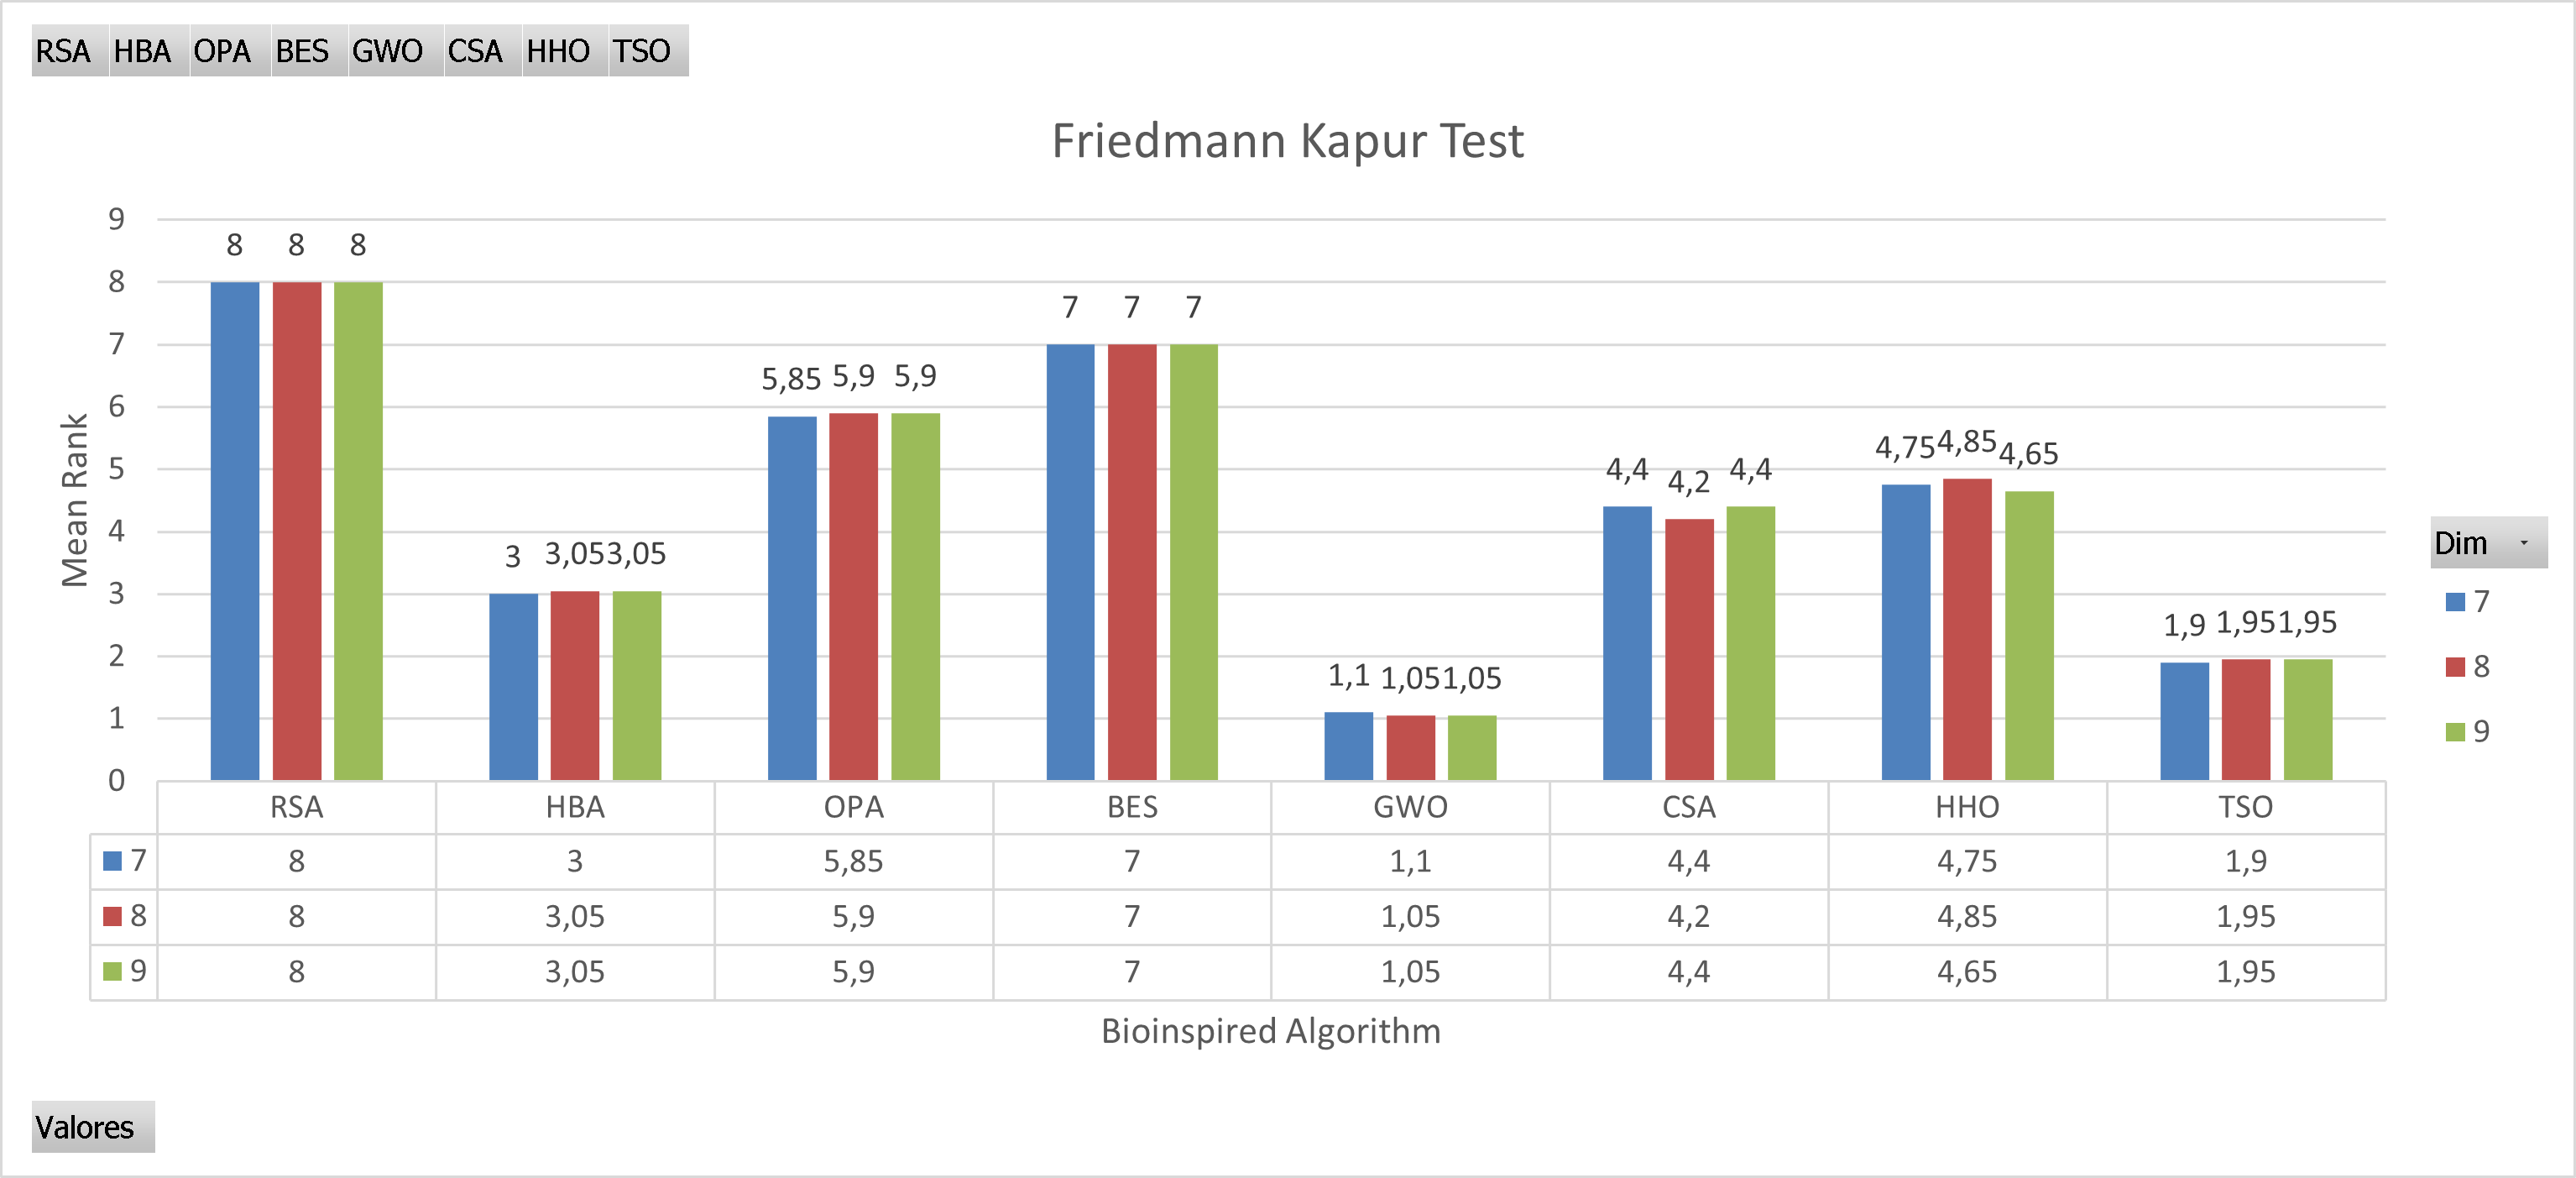
\includegraphics[width=0.8\textwidth]{Fitness/Kapur/Metrica_kapur_Friedman_results.png}
	\caption{Average fitness metric rank by dimension K and Kapur entropy objective function}
	\label{fig:Fitness_Kapur_Friedmann}
\end{figure}

\subsubsection{Función objetivo Otsu}
\noindent El analisis~\ref{fig:Fitness_Otsu_Friedmann} de los algoritmos GWO y TSO han demostrado ser excepcionalmente eficaces, sobresaliendo entre otros métodos evaluados. TSO mostró un rendimiento impresionante con rangos promedio de 1.5, 1.35 y 1.5 en las dimensiones 7, 8 y 9, respectivamente, indicando resultados consistentemente altos en todas las dimensiones evaluadas. De manera similar, GWO alcanzó los mejores rangos promedio en las mismas dimensiones, con 1.5 en las dimensiones 7 y 9, y 1.65 en la dimensión 8. Ambos algoritmos no solo se adaptan eficientemente según la métrica de aptitud y la función objetivo Otsu, sino que también ofrecen una robustez notable frente a variaciones en la dimensionalidad del problema.
\begin{figure}[H]
	\centering
	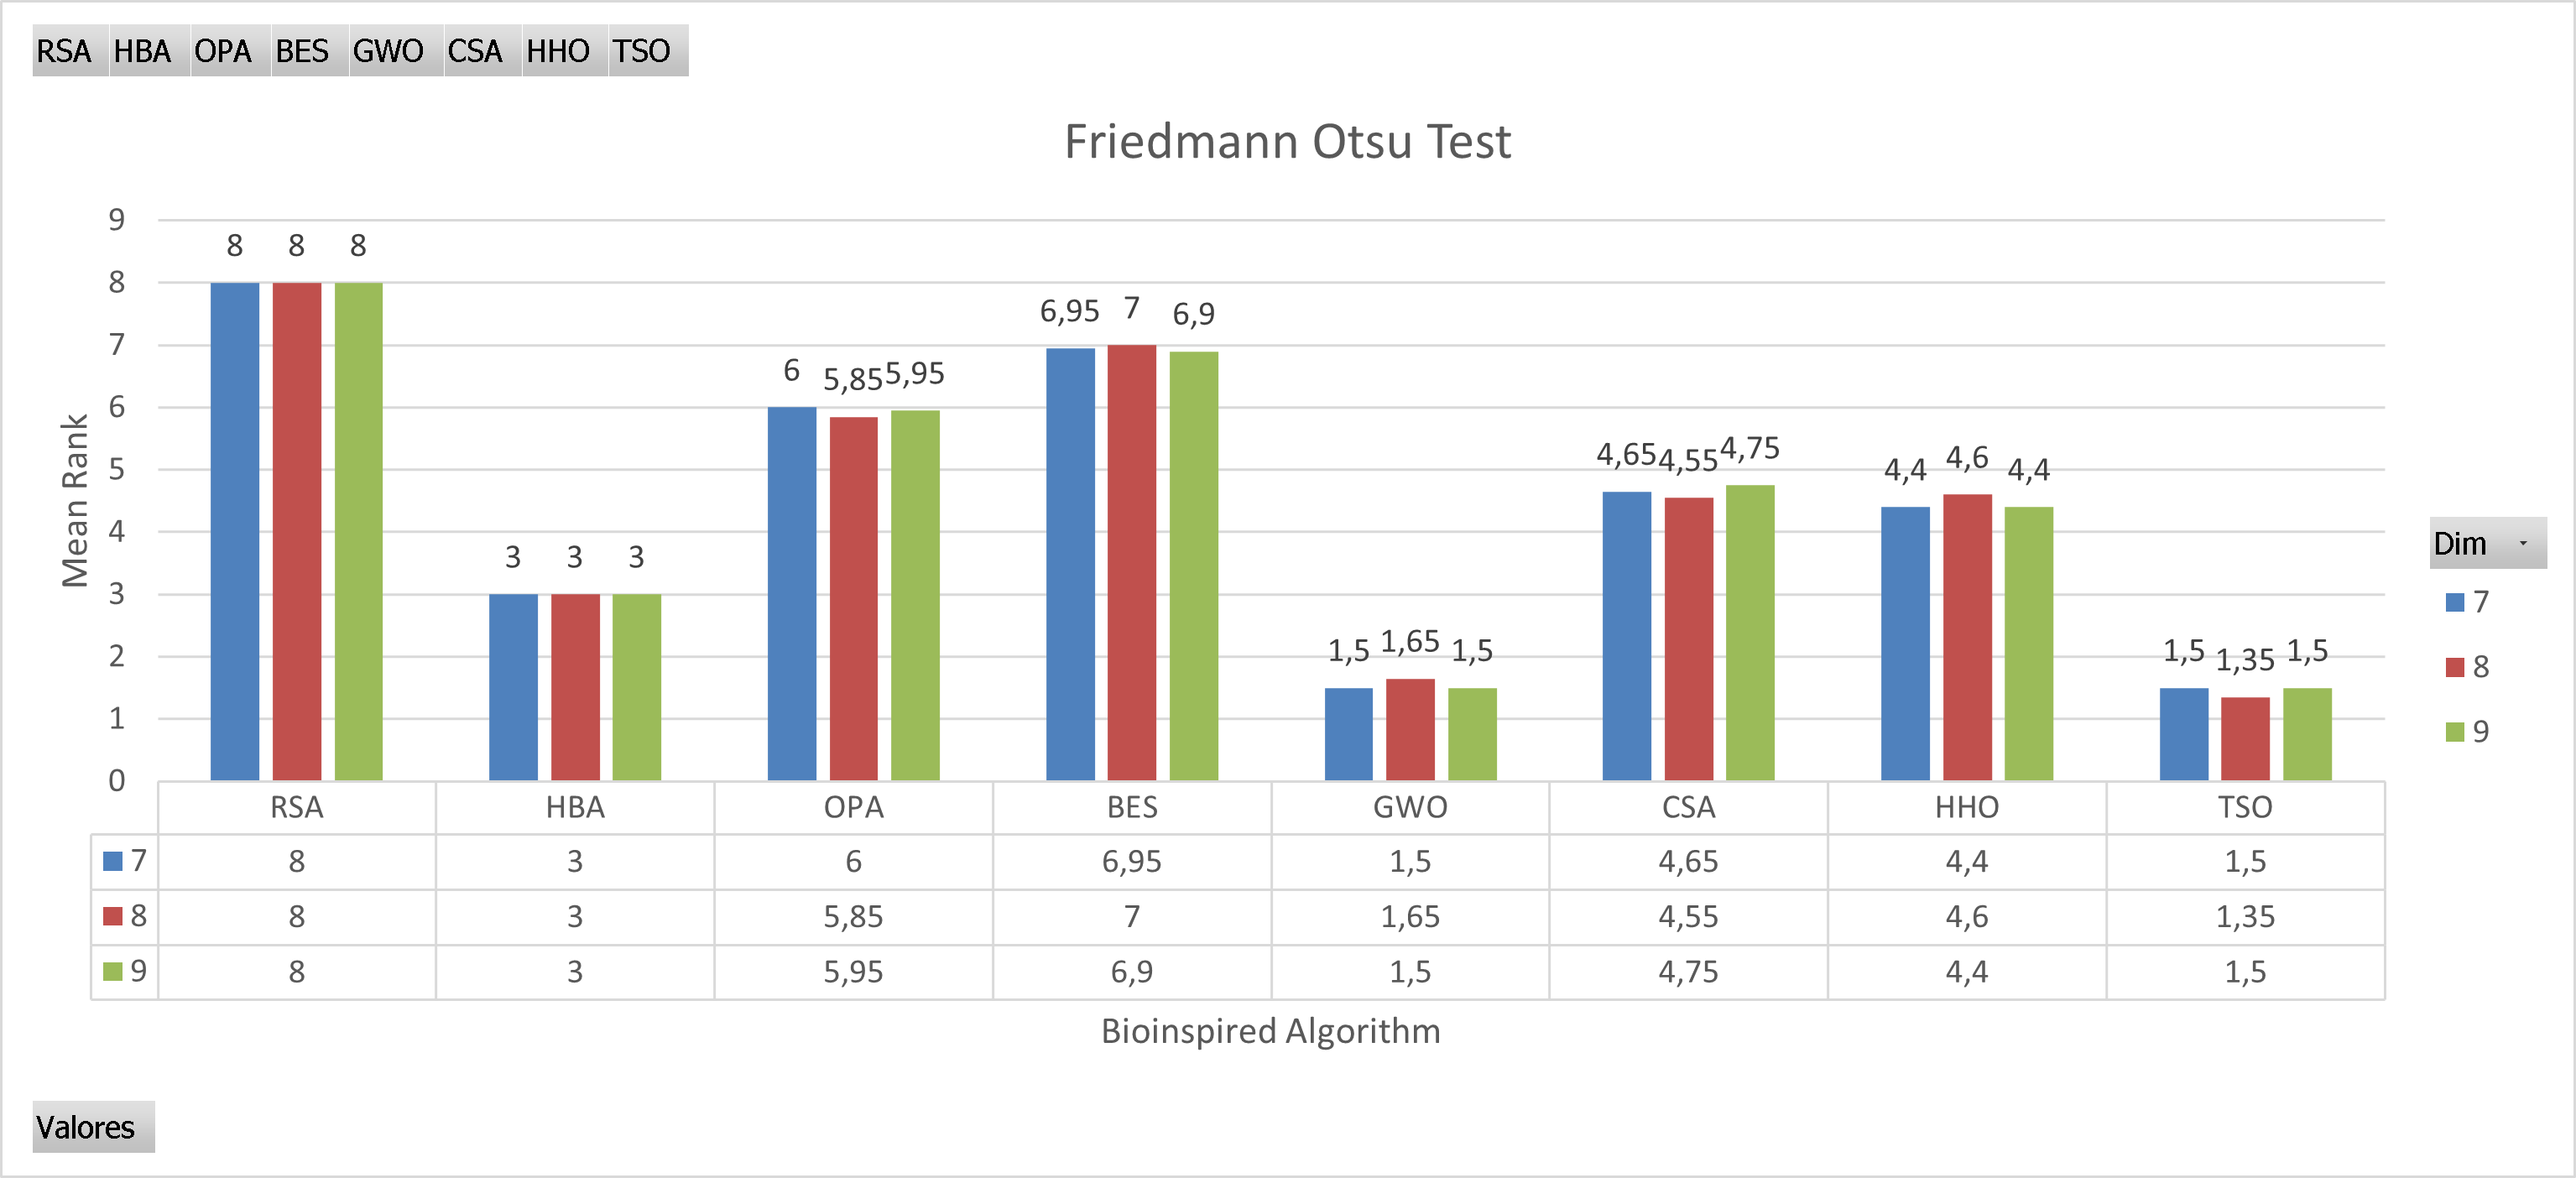
\includegraphics[width=0.8\textwidth]{Fitness/Otsu/Metrica_Otsu_Friedman_results.png}
	\caption{Average fitness metric rank by dimension K and Otsu objective function}
	\label{fig:Fitness_Otsu_Friedmann}
\end{figure}

\subsubsection{Función objetivo Tsallis}
\noindent El analisis~\ref{fig:Fitness_Tsallis_Friedmann}, los algoritmo GWO (Grey Wolf Optimizer) emergió como el más sobresaliente, logrando el rango promedio más bajo y el mejor desempeño con un resultado uniforme de 1.0 en todas las dimensiones evaluadas (7, 8 y 9). Esto demuestra su consistencia y superioridad en el test. Por su parte, el TSO también exhibió un excelente rendimiento, con un rango promedio constante de 2.0 en todas las dimensiones, posicionándose como el segundo mejor algoritmo.

\begin{figure}[H]
	\centering
	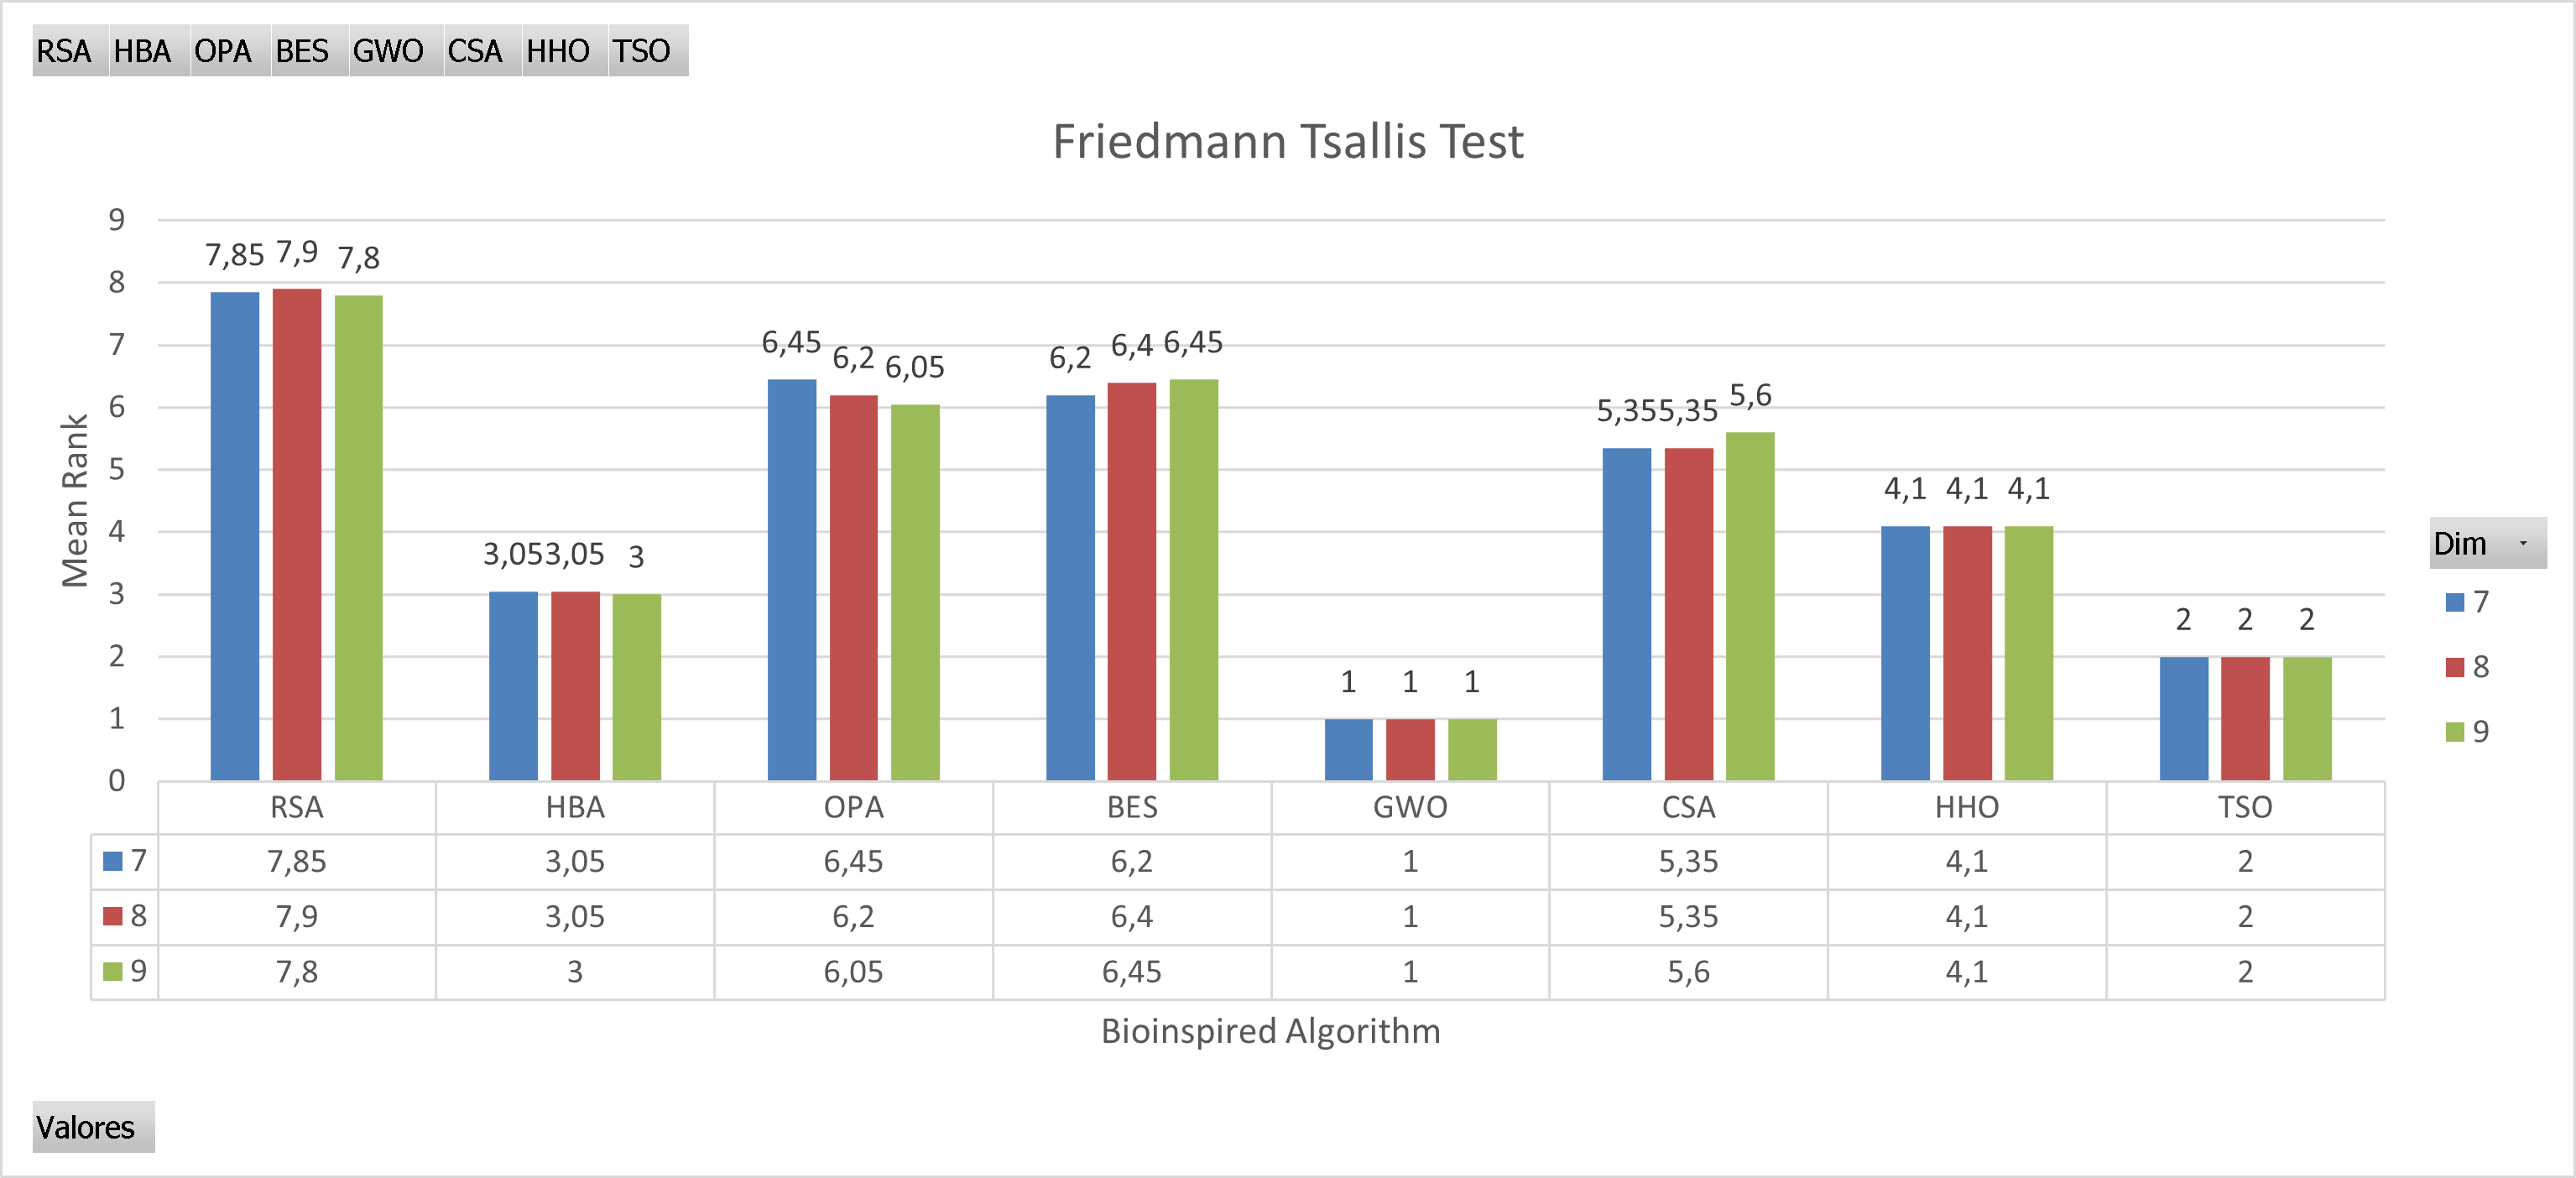
\includegraphics[width=0.8\textwidth]{Fitness/Tsallis/Metrica_Tsallis_Friedman_results.png}
	\caption{Average fitness metric rank by dimension K and Tsallis objective function}
	\label{fig:Fitness_Tsallis_Friedmann}
\end{figure}

\section{Discussion of Results} \label{sec:di}

\noindent Research on the segmentation of brain images using metaheuristic optimization algorithms has revealed fundamental aspects about the performance of these techniques in a highly specialized medical context. The results provide significant evidence of the efficacy of these algorithms, particularly the Grey Wolf Optimizer (GWO), in enhancing the quality and accuracy of magnetic resonance image segmentation.

\noindent The analysis of the algorithms under different metrics (fitness, PSNR, and SSIM) revealed that although there is variability in performance among the algorithms, some consistently stand out. For example, GWO demonstrated superior performance across almost all metrics and conditions, suggesting its robustness and adaptability to different types of images and segmentation requirements. This consistency is crucial in medical applications, where precision and reliability are of utmost importance for effective diagnosis and treatment.

\noindent The fitness function, which measures the quality of segmentation in terms of a predefined goal, was particularly useful for assessing how the algorithms optimize the segmentation process. The results showed that GWO and other algorithms such as the Honey Badger Algorithm (HBA) and Tuna Swarm Optimization (TSO) were able to effectively explore the search space, finding optimal or near-optimal solutions under various conditions. This exploration capability is essential to adapt to the natural variability present in medical images.

\noindent As for the PSNR, which measures the signal-to-noise ratio and hence the preservation of image quality, the results once again highlighted the efficacy of GWO and HBA. These algorithms not only achieved high PSNR values but also showed low variability in their performance, indicating consistent preservation of image quality across different samples. This feature is vital to ensure that segmentation does not degrade the essential information contained in medical images.

\noindent The SSIM, which assesses the structural similarity between the segmented image and the original, is another critical metric in medical image segmentation. Algorithms that achieved high SSIM values, such as GWO and HBA, demonstrated their ability to maintain the essential structural characteristics of the images, crucial for medical applications where the accuracy of anatomical structure is paramount.

\noindent The influence of dimension K on the performance of the algorithms was also examined. Although general improvements in segmentation quality with an increase in K were observed, no direct and uniform correlation between K and algorithm performance was found. This suggests that the choice of K must be carefully considered and tailored to each specific situation, balancing the need for precision with computational complexity.

\noindent The variability in algorithm performance across different images underscores the importance of careful algorithm selection and parameterization for each type of image. This is particularly relevant in a clinical setting, where images can vary significantly in terms of quality, type of tissue represented, and presence of pathologies.

\noindent Overall, the results of this study are promising for the application of metaheuristic optimization algorithms in the medical field. The outstanding performance of certain algorithms in the precise segmentation of brain opens new possibilities for the diagnosis and treatment of brain diseases. However, it is crucial to consider the limitations and challenges associated with applying these techniques, such as the need for fine-tuning and detailed evaluation for each specific case.

\section{Conclusion} \label{sec:co}

\noindent This research provides important insights into the use and efficacy of metaheuristic optimization algorithms in the segmentation of medical images. The results emphasize the need for careful selection and tuning of these algorithms to fully leverage their capabilities in medical contexts, thereby enhancing the quality of diagnosis and treatment of diseases related to brain parenchyma.

\noindent There are significant differences in terms of the fitness metric. The descriptive statistical analysis indicates that the GWO algorithm has the highest mean and the smallest standard deviation, suggesting stability in its results during the 30 executions for all images and their dimensions. Similarly, the TSO algorithm obtained quite similar results but presents a much higher standard deviation than GWO. The Friedman test provides sufficient evidence to determine that the GWO algorithm exhibits a significant difference in performance compared to the rest of the algorithms.

\noindent Regarding the PSNR metric, the descriptive statistical analysis does not provide relevant information for analyzing the performance of the algorithms. On the other hand, the Friedman test provides sufficient evidence to determine that the GWO, CSA, HBA, and OPA algorithms showed a significant difference in performance compared to the other algorithms in the PSNR metric for all 20 images and across all dimensions.

\noindent The analysis of the results for the SSIM metric using descriptive statistics positions the GWO algorithm as one of the most stable, given its high mean and low standard deviation. Similarly, the Friedman test indicates that GWO is the algorithm that obtained the highest rank value, followed by HBA and OPA, showing a significant difference in performance for the SSIM metric. These results are valid for all images and their dimensions.

\noindent Finally, it is concluded that the GWO algorithm exhibits the best overall performance. However, it is necessary to highlight that these results are subject to the nature of the data, the complexity of the images, and the context in which the brain image segmentation is used with the GWO algorithm.

\section{Appendix A}
\label{sec:appendix}
\noindent Due to the extent of the tables, results, and images generated in this study, they have been made available in external repositories for easy access and reference. The detailed results, including the application of the Friedman test to the three evaluation metrics (fitness, SSIM, PSNR), can be found at the following link: \url{https://doi.org/10.6084/m9.figshare.25709067}. These results complement the findings presented in this article and provide a comprehensive analysis of the performance of the metaheuristic algorithms in image segmentation.

\noindent The availability of these additional resources aims to foster reproducibility and transparency in our research, enabling other researchers to verify our findings and build upon them. We invite readers to explore these resources to gain a deeper understanding of the results presented in this article and their relevance to the field of medical image segmentation.
\section{Appendix B}
\label{sec:appendixB}
\begin{figure}[H]
    \centering
    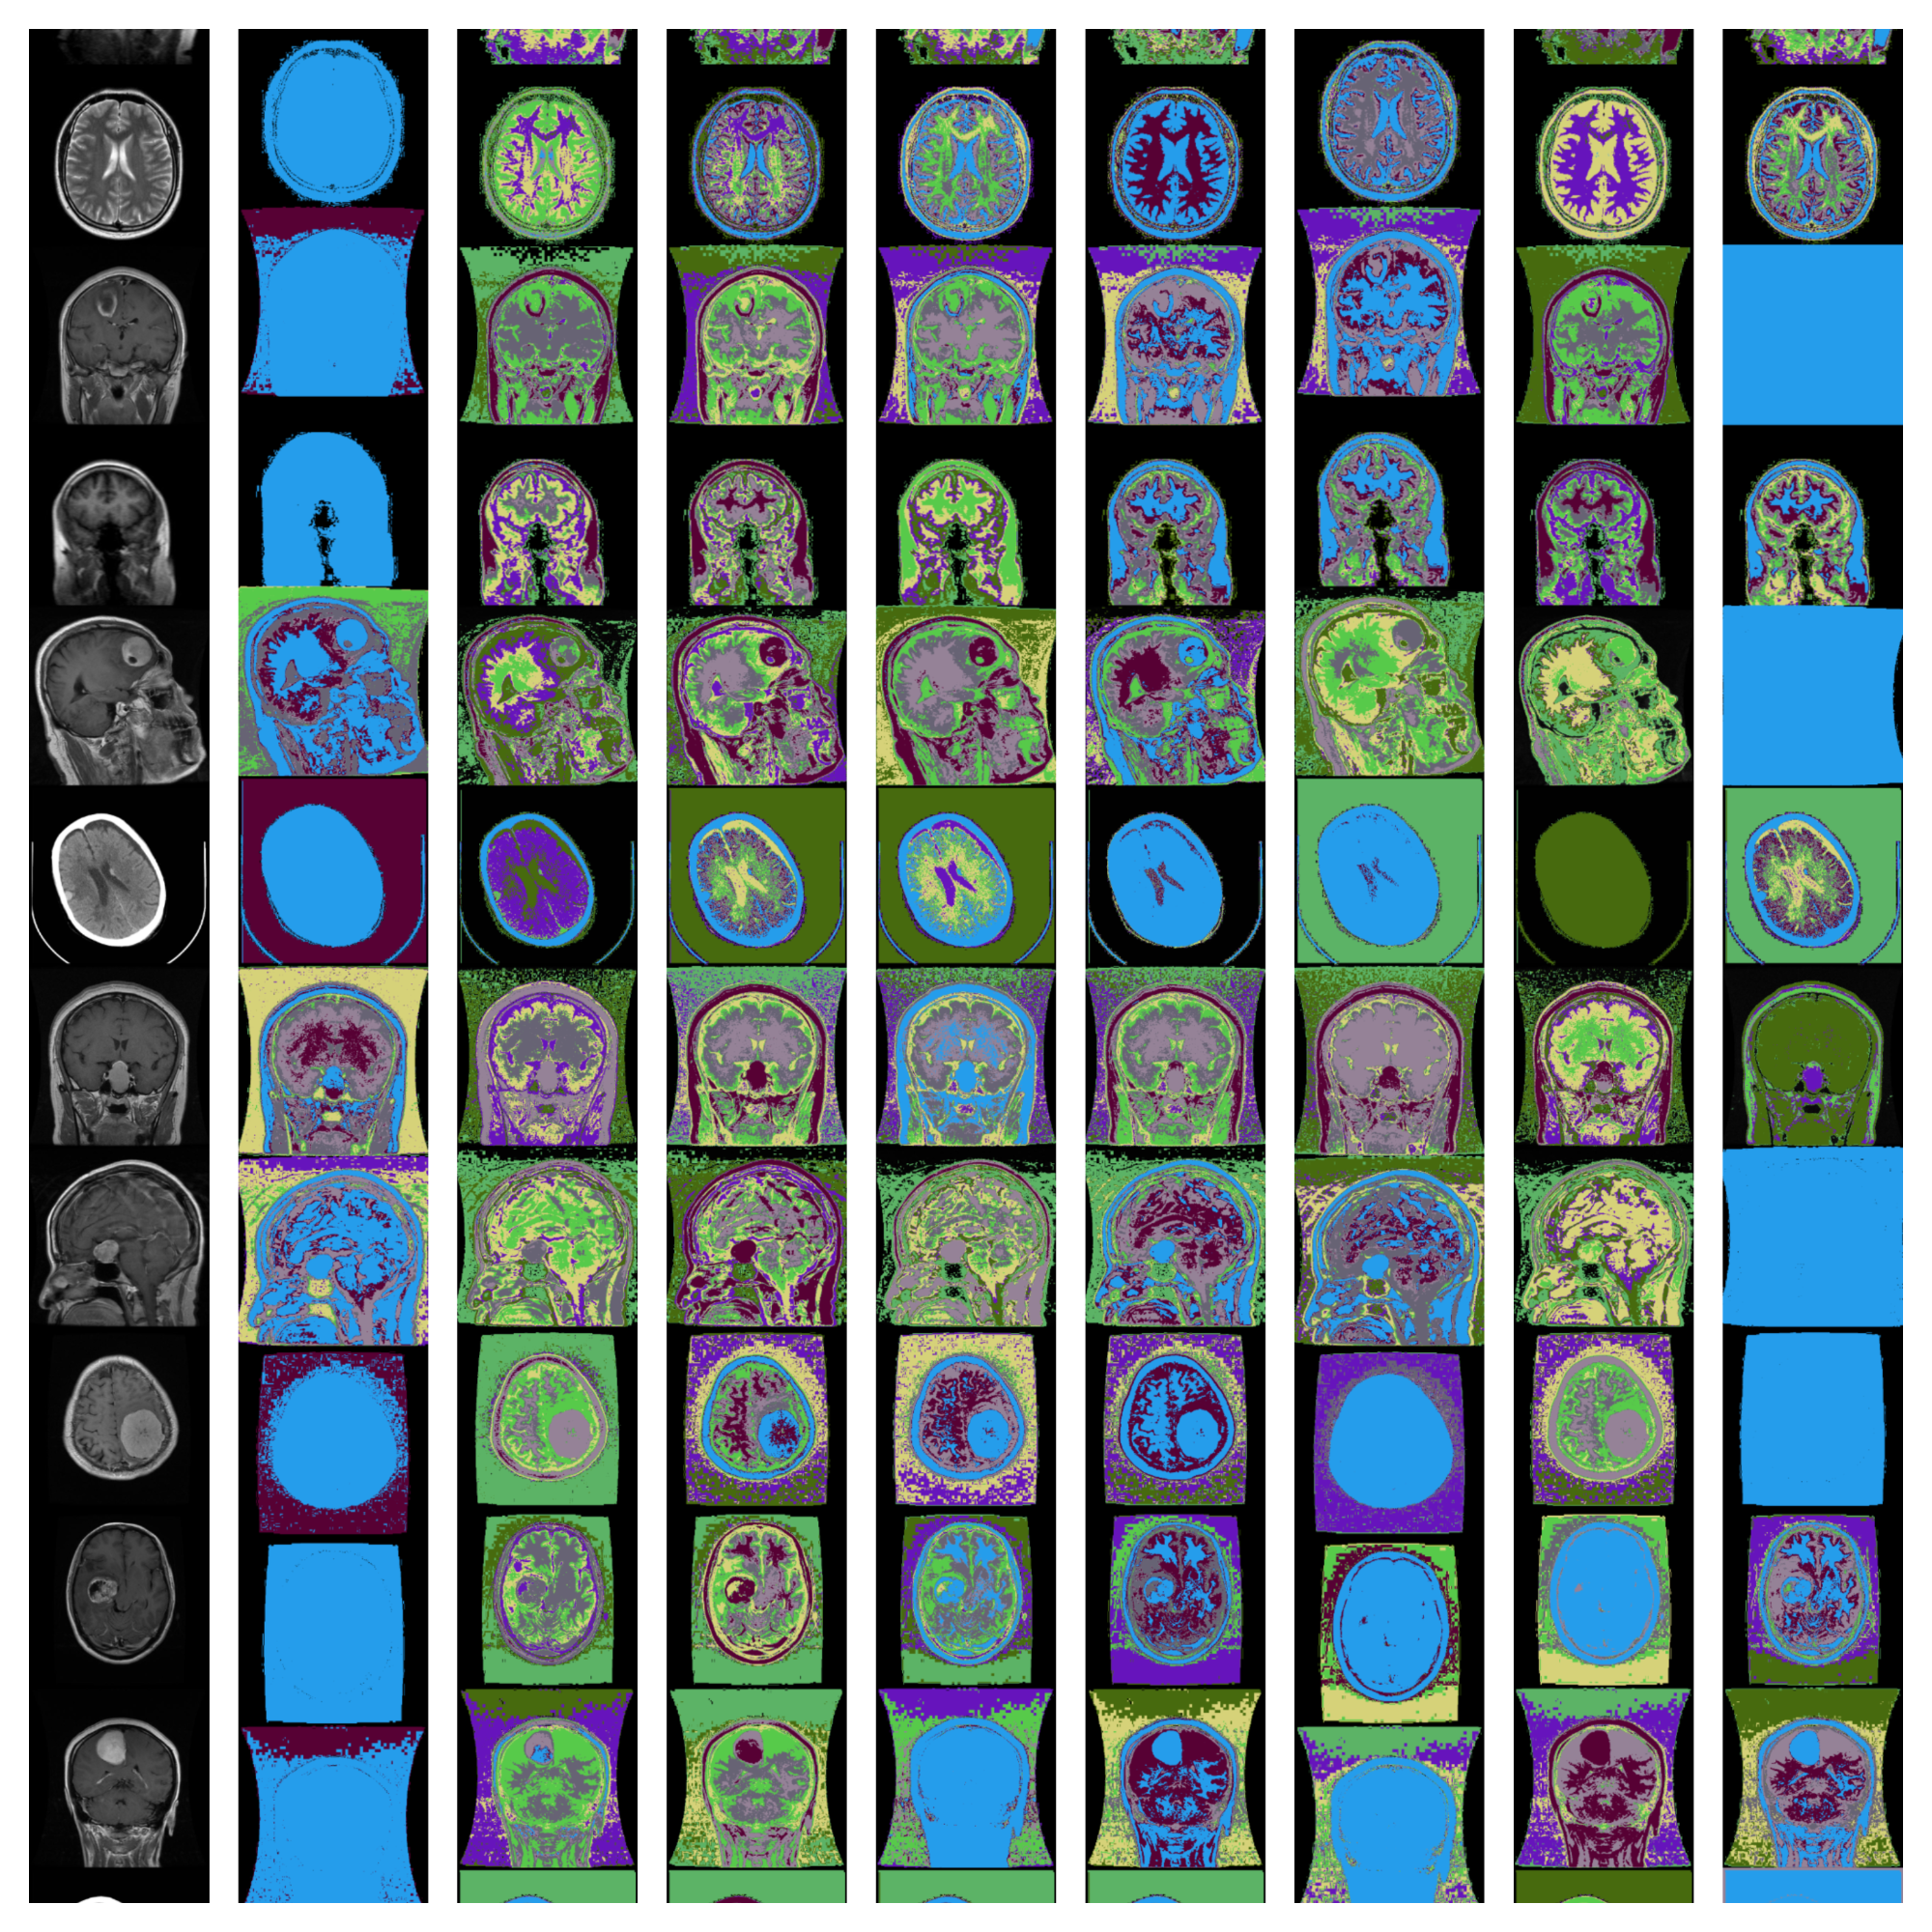
\includegraphics[width=0.6\textwidth]{img/Metrica_8_bits_9_dim_Tsallis_BES_umbral.png}
    \caption{Here is an example of the results obtained with the objective function based on Tsallis entropy, in K=9 dimensions and they are ordered from the original image to TSO in the following order:"RSA, HBA, OPA, BES, GWO, CSA, HHO, TSO."}
    \label{fig:Tsallis_Umbral}
\end{figure}
\begin{figure}[H]
    \centering
    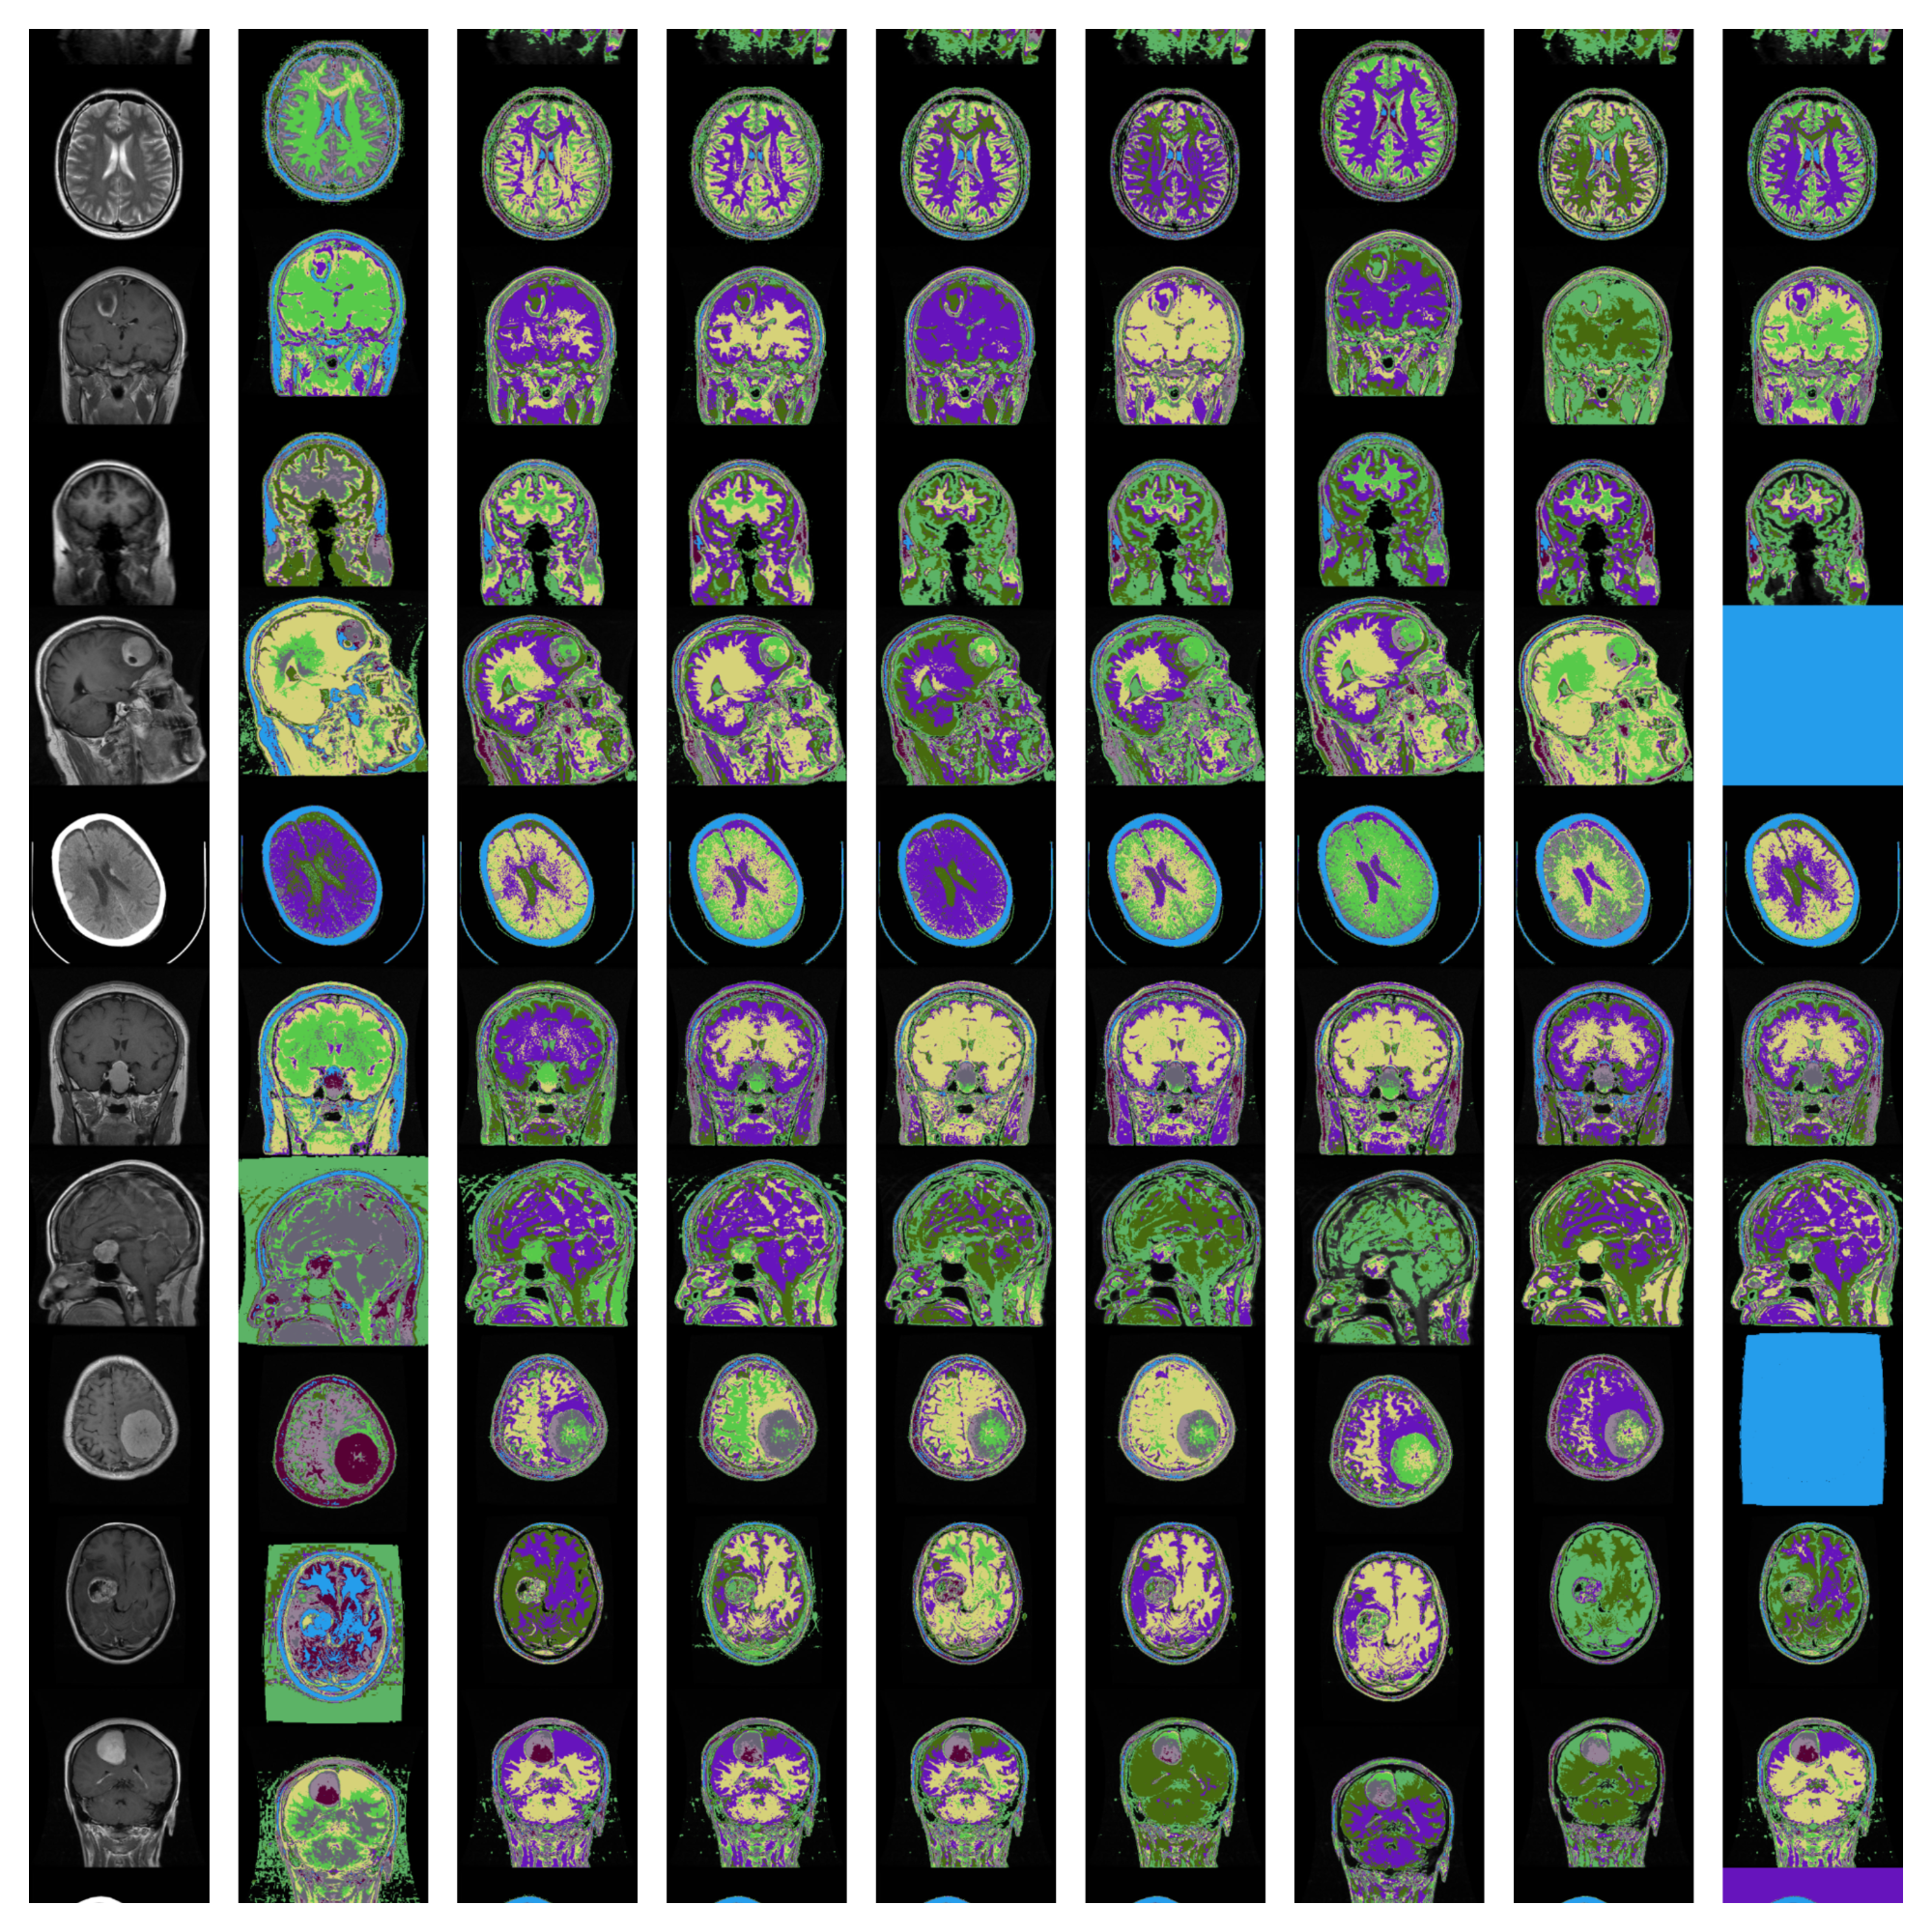
\includegraphics[width=0.6\textwidth]{img/Metrica_8_bits_9_dim_kapur_BES_umbral.png}
    \caption{Here is an example of the results obtained with the objective function based on Kapur´s entropy, in K=9 dimensions and they are ordered from the original image to TSO in the following order:"RSA, HBA, OPA, BES, GWO, CSA, HHO, TSO."}
    \label{fig:Kapur_Umbral}
\end{figure}
\begin{figure}[H]
    \centering
    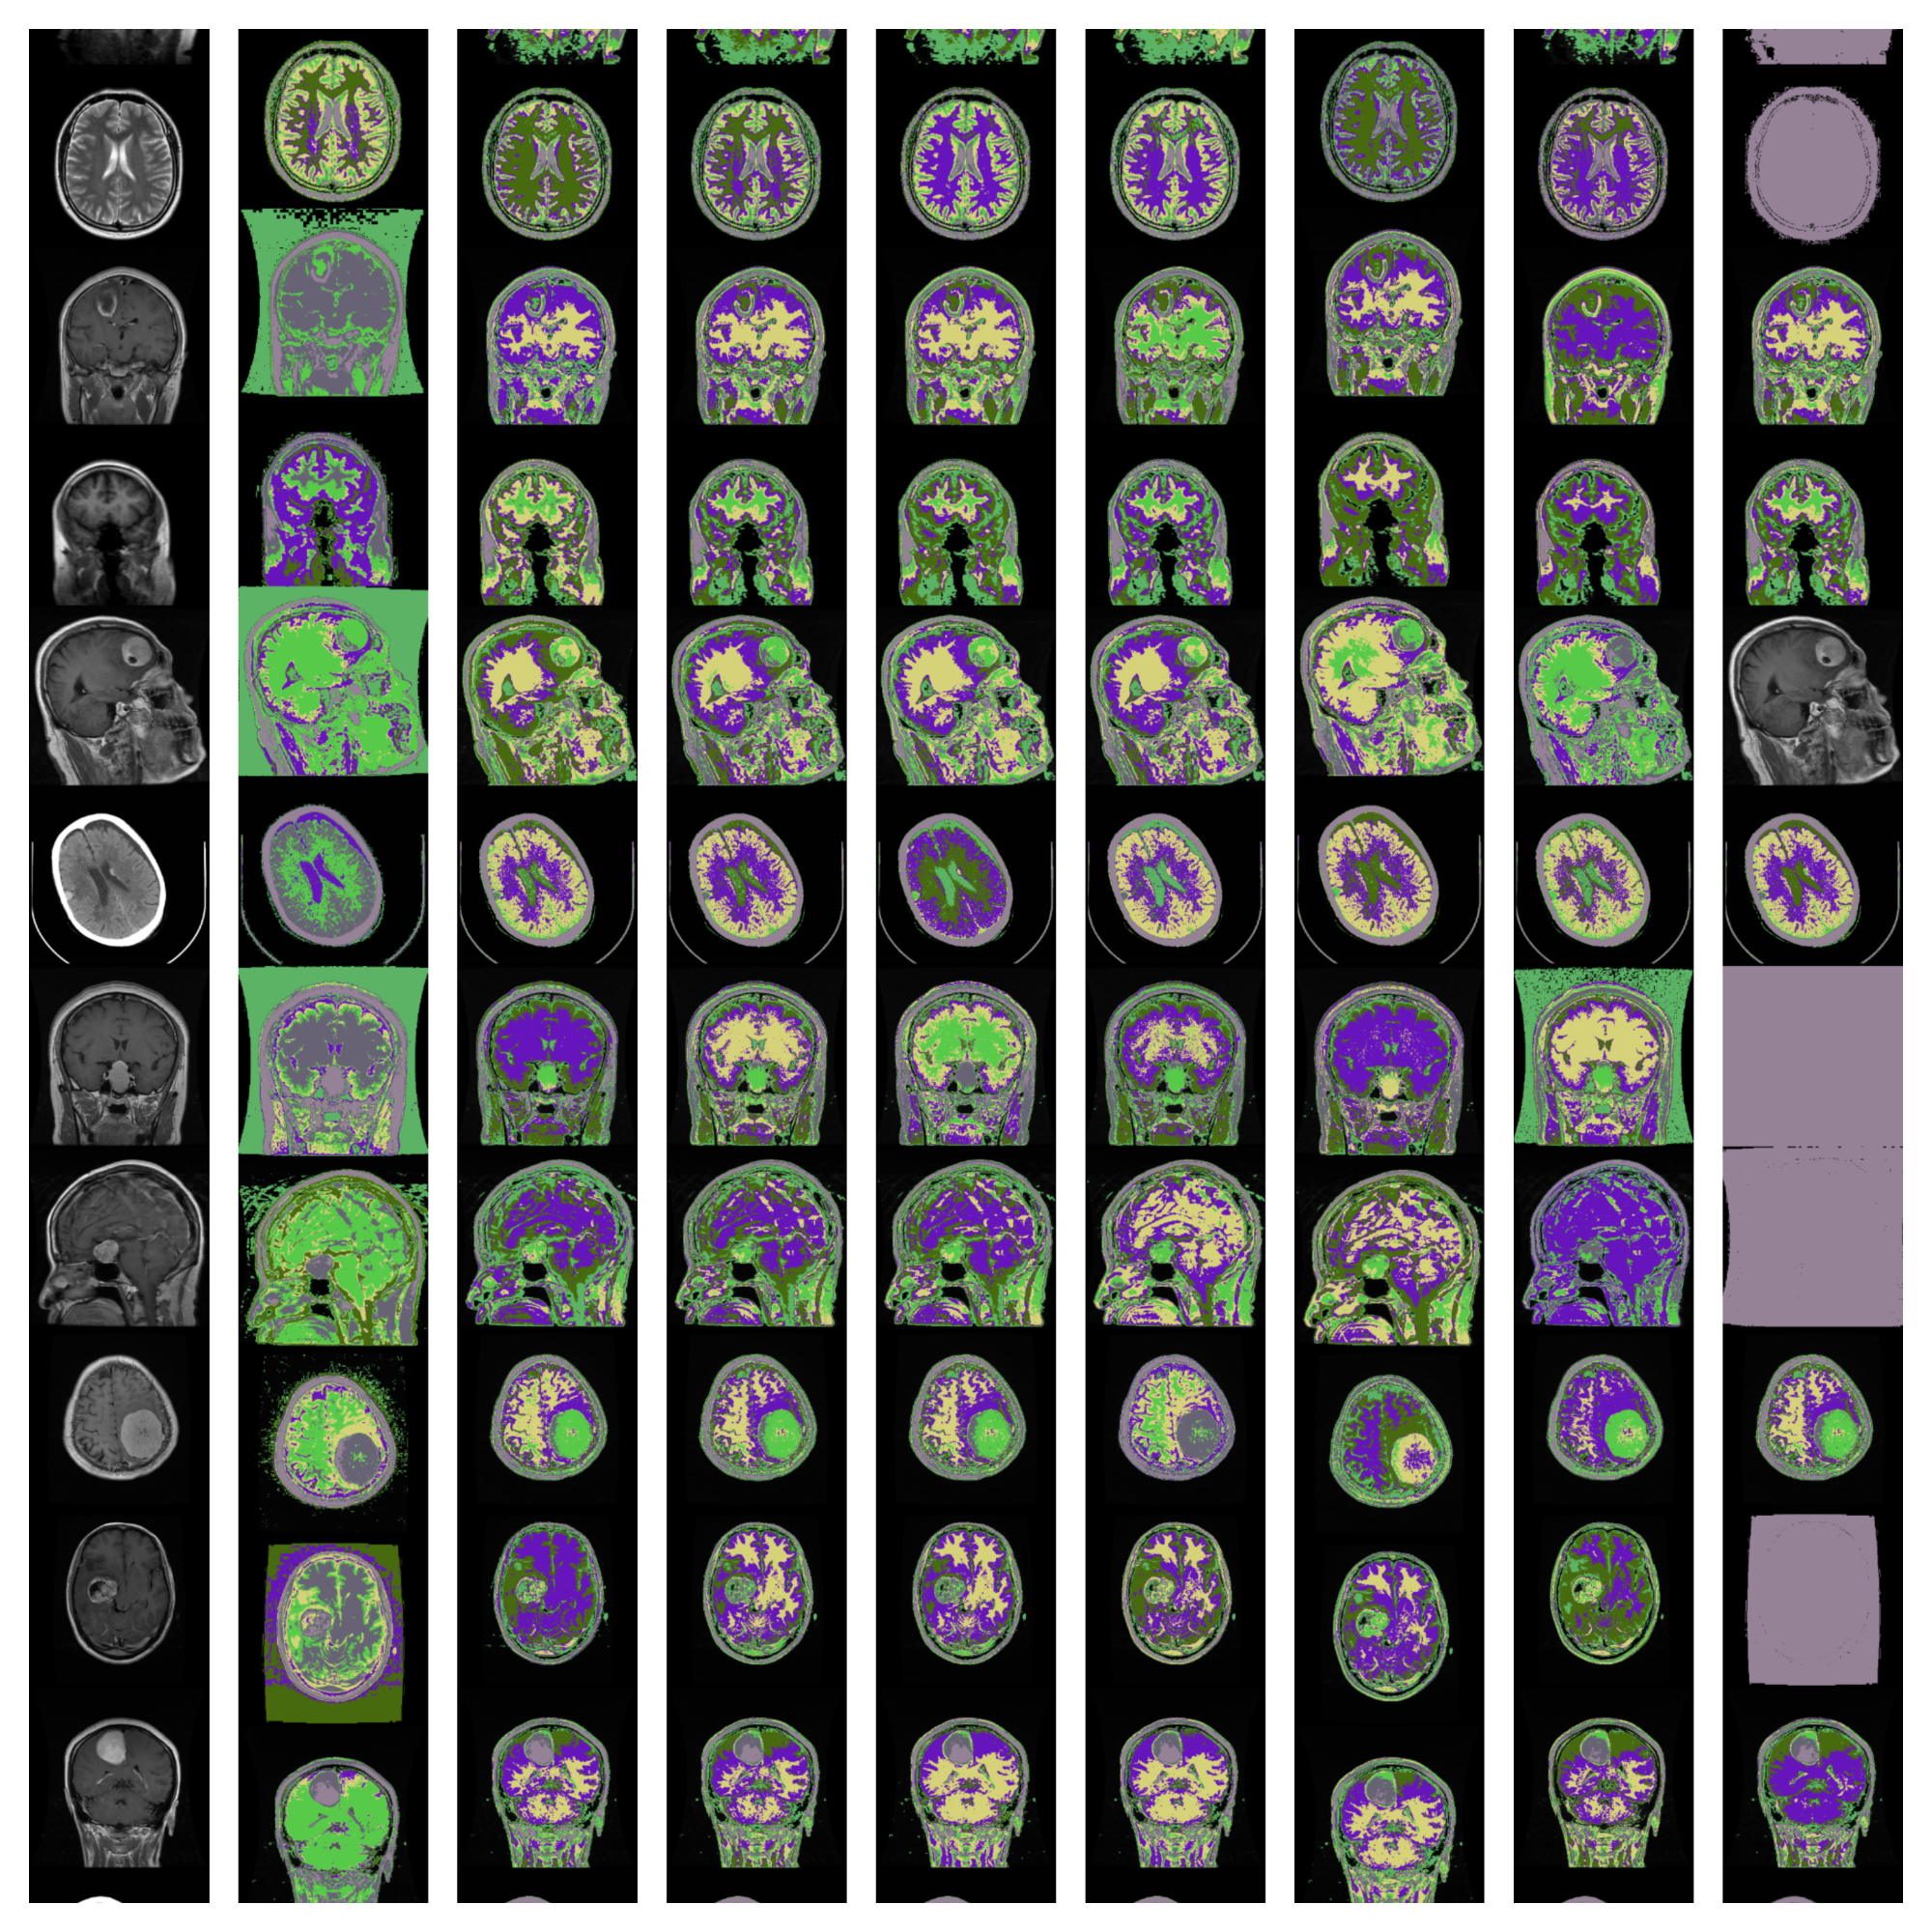
\includegraphics[width=0.6\textwidth]{img/Metrica_8_bits_9_dim_otsu_BES_umbral.png}
    \caption{Here is an example of the results obtained with the objective function based on Otsu Method, in K=9 dimensions and they are ordered from the original image to TSO in the following order:"RSA, HBA, OPA, BES, GWO, CSA, HHO, TSO."}
    \label{fig:Otsu_Umbral}
\end{figure}

\bibliographystyle{elsarticle-num}
\bibliography{references}
\end{document}